% PDF profiles from one source (V7).
%   interactive: blue mailto/DOI/URL links and a clickable ORCID logo.
%   ieee (default): no link annotations and no bookmarks, for IEEE PDF eXpress;
%   metadata written with \pdfinfo; ORCID logo kept as plain vector art.
% Select with \def\PDFPROFILE{interactive} before % IEEE conference format, same structure as the group's HRFEST papers 223 and 235.
% Every number in the text comes from tables/values.tex, generated from results/.
%   \def\PDFPROFILE{ieee}   no link annotations, for IEEE PDF eXpress
\ifdefined\PDFPROFILE\else\def\PDFPROFILE{interactive}\fi
\ifdefined\SIMFIGURE\else\def\REALPHOTOS{}\fi  % Fig. 1 shows the physical robot; \def\SIMFIGURE{} uses MuJoCo renders
\documentclass[conference,a4paper]{IEEEtran}
\IEEEoverridecommandlockouts
\usepackage[a4paper,top=36mm,bottom=19mm,left=19mm,right=19mm]{geometry}  % the IEEE-EPIC author page
\usepackage{balance}
\usepackage{placeins}
\usepackage[utf8]{inputenc}
\usepackage[T1]{fontenc}
\usepackage{cite}
\usepackage{graphicx}
\usepackage{amsmath,amssymb}
\usepackage{booktabs}
\usepackage{microtype}
\usepackage{url}
\usepackage{xcolor}
\newcommand{\PaperTitle}{Proprioception-Augmented Risk Mapping for a Commercial Quadruped: Terrain-Aware Navigation Across Legged and Wheeled Configurations}
\newcommand{\PaperAuthors}{Jose Luis Segundo Manayay, Javier Yanpier Garay Yovera, Francisco Jes\'us Rodr\'iguez Huiman}
\newcommand{\PaperAuthorsPDF}{Jose Luis Segundo Manayay, Javier Yanpier Garay Yovera, Francisco Jes\string\372s Rodr\string\355guez Huiman}
% PDF profiles from one source (V7).
%   interactive: blue mailto/DOI/URL links and a clickable ORCID logo.
%   ieee (default): no link annotations and no bookmarks, for IEEE PDF eXpress;
%   metadata written with \pdfinfo; ORCID logo kept as plain vector art.
% Select with \def\PDFPROFILE{interactive} before % IEEE conference format, same structure as the group's HRFEST papers 223 and 235.
% Every number in the text comes from tables/values.tex, generated from results/.
%   \def\PDFPROFILE{ieee}   no link annotations, for IEEE PDF eXpress
\ifdefined\PDFPROFILE\else\def\PDFPROFILE{interactive}\fi
\ifdefined\SIMFIGURE\else\def\REALPHOTOS{}\fi  % Fig. 1 shows the physical robot; \def\SIMFIGURE{} uses MuJoCo renders
\documentclass[conference,a4paper]{IEEEtran}
\IEEEoverridecommandlockouts
\usepackage[a4paper,top=36mm,bottom=19mm,left=19mm,right=19mm]{geometry}  % the IEEE-EPIC author page
\usepackage{balance}
\usepackage{placeins}
\usepackage[utf8]{inputenc}
\usepackage[T1]{fontenc}
\usepackage{cite}
\usepackage{graphicx}
\usepackage{amsmath,amssymb}
\usepackage{booktabs}
\usepackage{microtype}
\usepackage{url}
\usepackage{xcolor}
\newcommand{\PaperTitle}{Proprioception-Augmented Risk Mapping for a Commercial Quadruped: Terrain-Aware Navigation Across Legged and Wheeled Configurations}
\newcommand{\PaperAuthors}{Jose Luis Segundo Manayay, Javier Yanpier Garay Yovera, Francisco Jes\'us Rodr\'iguez Huiman}
\newcommand{\PaperAuthorsPDF}{Jose Luis Segundo Manayay, Javier Yanpier Garay Yovera, Francisco Jes\string\372s Rodr\string\355guez Huiman}
\input{profile}
\usetikzlibrary{arrows.meta,backgrounds,fit,calc}
\definecolor{amberfill}{HTML}{FBEFC9}
\definecolor{greenfill}{HTML}{E3F1EC}
\urlstyle{same}
\input{tables/values.tex}
\renewcommand{\topfraction}{0.92}
\renewcommand{\bottomfraction}{0.85}
\renewcommand{\textfraction}{0.07}
\renewcommand{\floatpagefraction}{0.80}
\setlength{\textfloatsep}{7pt plus 2pt minus 2pt}
\setlength{\floatsep}{7pt plus 2pt minus 2pt}
\setlength{\intextsep}{7pt plus 2pt minus 2pt}
\setlength{\abovecaptionskip}{3pt}
\setlength{\belowcaptionskip}{0pt}

\clubpenalty=10000
\widowpenalty=10000
\displaywidowpenalty=10000
\newcommand{\sentbreak}{\par\pagebreak\noindent}  % a column ends only at the end of a sentence (scripts/fix_breaks.py)

% Fixed heading space: a column that ends early spreads its gap over all its lines, a fraction of a point each.
\makeatletter
\def\section{\@startsection{section}{1}{\z@}{1.5ex}{0.7ex}{\normalfont\normalsize\centering\scshape}}
\def\subsection{\@startsection{subsection}{2}{\z@}{1.2ex}{0.5ex}{\normalfont\normalsize\itshape}}
\makeatother
\setlength{\parskip}{0pt}
\flushbottom
\AtBeginDocument{\setlength{\baselineskip}{12pt plus 0.8pt}}

\begin{document}

\title{Proprioception-Augmented Risk Mapping for a Commercial Quadruped: Terrain-Aware Navigation Across Legged and Wheeled Configurations}

\author{\IEEEauthorblockN{Jose Luis Segundo Manayay\,\orcid{0009-0002-9203-8710},
Javier Yanpier Garay Yovera\,\orcid{0009-0001-1645-8724},
Francisco Jes\'us Rodr\'iguez Huiman\,\orcid{0009-0006-6972-2484}}
\IEEEauthorblockA{Universidad Nacional de Ingenier\'ia (UNI), Faculty of Mechanical Engineering, Lima, Peru\\
\authoremail{jose.segundo.m@uni.pe}; \authoremail{javier.garay.y@uni.pe}; \authoremail{francisco.rodriguez.h@uni.pe}}}

\maketitle

\begin{abstract}
Inspection robots build risk maps from geometry, yet slippery or soft ground can look as flat as concrete. This paper studies how proprioceptive evidence should enter a risk map, and whether its value depends on the foot configuration of a commercial quadruped, the DOBOT Rover X1, whose legged and wheeled configurations are fixed before a mission. In MuJoCo, \vnEpisodesTotal{} dynamic episodes on parametrised terrain train a lightweight classifier and measure falls per metre. A separate Monte Carlo study compares geometry-only mapping, local Bayesian updating, appearance-based propagation and an uncertainty-aware fusion on 200 procedural indoor maps with paired statistics. Propagation raised mission survival probability by 0.055 over local updating and fusion added 0.015; both effects held on 200 independent maps, while local updating was practically indistinguishable from geometry. In simulation the legged robot fell on low-friction and soft terrain and the wheeled model never fell, so the benefit of propagation followed the failure model, not perception quality. The classifier reached macro-F1 of 0.935 and 0.999 on held-out episodes but dropped to 0.45 for the legged robot at unseen speeds. All results are simulation only; appearance features remain assumed and no hardware validation is claimed.
\end{abstract}

\begin{IEEEkeywords}
legged robots, wheeled-legged robots, proprioception, terrain classification, traversability, risk-aware planning, Monte Carlo simulation
\end{IEEEkeywords}

\section{Introduction}
Autonomous inspection of underground and industrial spaces depends on knowing which ground can be crossed. Quadrupeds have operated in such settings~\cite{tranzatto2022,gao2026}, but geometry says little about friction or softness: a wet floor and dry concrete return the same LiDAR profile, and the robot learns the difference only on contact. Commercial quadrupeds expose joint and inertial signals that could reveal it, behind closed locomotion controllers.

This raises a question separate from the classifier itself: \emph{how should a proprioceptive detection enter the planner's risk map?} It can update only the ground already crossed, or generalise to unvisited ground that looks alike. A second question is whether the answer depends on the feet. The DOBOT Rover X1 uses point-foot and wheel modules that are exchanged by hand (Fig.~\ref{fig:quadrupeds}), so the configuration is fixed before a mission; we treat them as two robots and model no switching.

\begin{figure}[!t]
\centering
\ifdefined\REALPHOTOS
{\scriptsize\setlength{\tabcolsep}{1.5pt}\begin{tabular}{cc}
(a) Legged & (b) Wheeled\\
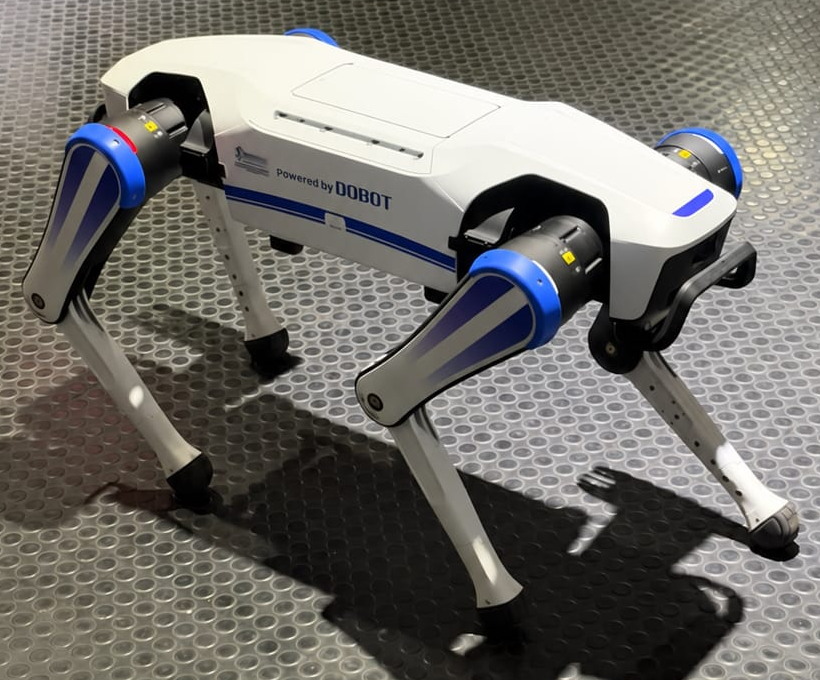
\includegraphics[height=28mm]{figures/photos/robot_legged.png} & 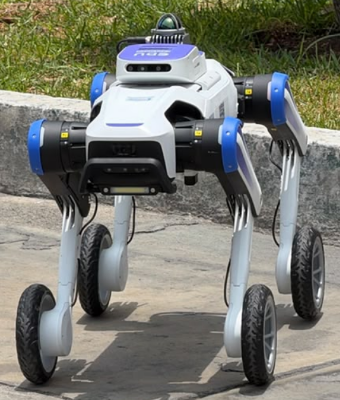
\includegraphics[height=28mm]{figures/photos/robot_wheeled.png}
\end{tabular}}
\caption{The physical DOBOT Rover X1: (a) legged, with point feet; (b) wheeled, with wheel modules. The modules are exchanged by hand, so each mission uses one configuration. The results of this paper come from simulation, not from these scenes.}
\else
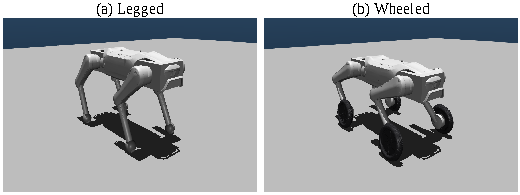
\includegraphics[width=\columnwidth]{figures/fig0_quadrupeds.pdf}
\caption{The two configurations studied, as MuJoCo simulation renders, not photographs: (a) legged, with point feet and 12 actuators; (b) wheeled, with wheel modules and 16 actuators. On the robot the modules are exchanged by hand, so each mission uses one configuration.}
\fi
\label{fig:quadrupeds}
\end{figure}

Comparisons of this kind risk circularity: if failure rates are assumed to differ between wheels and legs, finding that the benefit differs restates the assumption. \sentbreak We therefore separate perception from failure and measure both in dynamic simulation where possible. Our contributions are:
\begin{enumerate}
\item A reproducible, paired Monte Carlo comparison of four map-update rules, with independent repetition and sensitivity analysis.
\item A dynamic-simulation dataset of both configurations on parametrised terrain, and a lightweight classifier stress-tested beyond its training range.
\item Evidence that the failure model decides how the benefit depends on the feet: simulated falls reverse which configuration gains.
\end{enumerate}
This work follows our inspection architecture on a small servo-driven platform~\cite{segundo2026laccei}, but addresses a different question on a different robot. We claim no novelty for the fusion rule, a tempered Bayesian update of known form~\cite{bissiri2016}.

\begin{figure*}[t]
\centering
\resizebox{\textwidth}{!}{\input{figures/fig_study.tex}}
\caption{Study structure. Dynamic simulation supplies the classifier, its held-out confusion and fall rates; these enter the algorithmic Monte Carlo offline, where each method sees only its own observations. Colour gives the status of each block.}
\label{fig:arch}
\end{figure*}

\section{Related Work}
Wheels on a quadruped can greatly reduce the cost of transport~\cite{bjelonic2019}, and learned controllers achieve robust hybrid navigation~\cite{lee2024}, but those systems own their controller; here perception and planning act above a closed one. Terrain can be classified from foot forces and joint signals~\cite{bednarek2019}, soils inspected haptically~\cite{kolvenbach2019}, compliance estimated online for control~\cite{fahmi2020}, and traversability estimated from legged proprioception~\cite{elnoor2024}. We ask instead how such an estimate should spread through a map. Self-supervised methods project proprioceptive labels onto images~\cite{wellhausen2019}, Wild Visual Navigation learns traversability online from visual features~\cite{mattamala2025}, and terrain-property maps combine semantics with proprioceptive estimates~\cite{ewen2022}. Those works use real robots and images, which we do not. \sentbreak Our addition is narrower: a paired measurement of what propagation is worth as classification error and appearance ambiguity vary. Risk-aware planners use CVaR over traversability~\cite{fan2021} or evidential uncertainty~\cite{cai2024}; our simpler planner is only a common testbed.

\begin{figure*}[t]
\centering
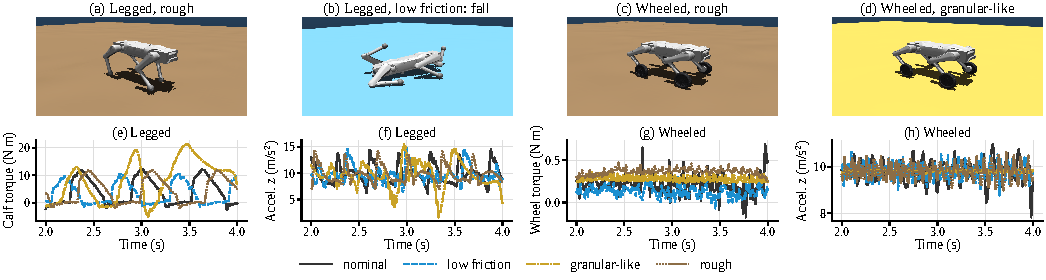
\includegraphics[width=\textwidth]{figures/fig9_mujoco.pdf}
\caption{MuJoCo simulation. (a)--(d) Renders of campaign episodes, with floor colour added for display only. (e)--(h) Logged signals over 2\,s on the four terrains, from example episodes that lasted at least 5.5\,s. Commanded torque is the actuator command, not a contact force.}
\label{fig:mujoco}
\end{figure*}
\section{Platform and Simulation Models}
The manufacturer specifies 15.5\,kg with point feet and 18.5\,kg with wheels, a Livox Mid-360 LiDAR, a RealSense D435i and a Jetson Orin Nano. Dynamics use MuJoCo~\cite{todorov2012} with models built from the manufacturer's files (the study is outlined in Fig.~\ref{fig:arch} and its control structure in Fig.~\ref{fig:control}). The legged model has 12 actuators and walks on the manufacturer's trained policy; the wheeled model has 16 and rolls on a skid-steer controller written for the project, because the manufacturer's is not public. The models weigh 18.65 and 22.08\,kg, not rescaled because the source of the difference is unknown. They are not calibrated digital twins.

Validating the models changed the setup. At the project's 200\,Hz control rate, the wheeled stance PD (400\,N\,m/rad, 7\,N\,m\,s/rad) produced a numerical limit cycle of about 70\,m/s$^2$ RMS at the IMU, even on a plane, which a classifier would learn as an artefact. We run physics and the stance PD at 1\,kHz, as a joint servo would; mean vertical contact force then matches model weight within 1\,\% on nominal terrain. The floor has contact priority, since MuJoCo otherwise uses the larger friction of a pair.

\begin{figure}[t]
\centering
\resizebox{\columnwidth}{!}{\input{figures/fig_control.tex}}
\caption{Control structure. The inner loop runs in MuJoCo; $y$ is the proprioceptive output. The outer loop runs in the Monte Carlo and is joined to the inner loop offline (dashed), through the classifier's confusion. The two were not closed online in one simulator.}
\label{fig:control}
\end{figure}

\section{Method}
\emph{Hazard.} A mission crosses terrain of true class $t_k\in\mathcal{T}=\{$nominal, low friction, granular-like, rough$\}$ over segments $\ell_k$. With per-metre hazard $h(t)$ and a patch multiplier $m_k$, survival is
\begin{equation}
P_s=\exp(-H),\qquad H=\sum_k \ell_k\, m_k\, h(t_k),
\label{eq:survival}
\end{equation}
since independent exponential failure times have additive hazards. $P_s=0$ if the goal is not reached within three times the shortest path. The hazard is a failure model, distinct from the classifier, and is never derived from F1.

\emph{Belief.} Each cell $i$ holds $b_i(t)$. Geometry observes relief only, so the prior separates rough terrain and nothing else:
\begin{equation}
b_i^0(t)\propto \pi(t)\,\mathcal{N}(r_i;\mu_t,\sigma_g^2).
\label{eq:prior}
\end{equation}
Every travelled window of $\ell_w$ metres yields a classifier output $o$ and confidence bin $c$, with likelihood $\hat p(o\mid t,c)$ estimated on calibration episodes. It is the add-half estimate
\begin{equation}
\hat p(o\mid t,c)=\frac{n_{t,o,c}+\tfrac12}{\sum_{o'}n_{t,o',c}+\tfrac12|\mathcal{T}|},
\label{eq:confusion}
\end{equation}
with $n_{t,o,c}$ the count of calibration windows of class $t$, output $o$ and confidence bin $c$ (maximum class probability below or above 0.8). Windows are assumed conditionally independent given $t$, which is optimistic and motivates the tempering below.

\emph{Update rules.} \textbf{M0} keeps \eqref{eq:prior}. \textbf{M1} applies Bayes' rule only to the cells of the traversed window:
\begin{equation}
b_i(t)\leftarrow b_i(t)\,\hat p(o\mid t,c)\Big/\sum\nolimits_{t'} b_i(t')\,\hat p(o\mid t',c).
\label{eq:bayes}
\end{equation}
\textbf{M2} is an online appearance vote. With kernel $s_i^w=\exp(-\lVert a_i-\bar a_w\rVert^2/2\sigma_k^2)$ between the appearance feature of cell $i$ and the mean feature of window $w$, votes are $V_i(k)=\sum_w s_i^w\mathbf{1}[o_w=k]$. Where $\sum_k V_i(k)\geq\tau$, the belief is replaced by the winning label, taken as correct. \textbf{M3} instead applies a tempered update,
\begin{equation}
\begin{aligned}
\log b_i(t)={}&\log b_i^0(t)+D_i(t)\\
&+\max\bigl[P_i(t)-\max\nolimits_{t'}P_i(t'),\,-C\bigr]+\text{const},
\end{aligned}
\label{eq:m3}
\end{equation}
where $D_i$ sums the log-likelihoods of windows that crossed cell $i$ and $P_i(t)=\rho\sum_w s_i^w\log\hat p(o_w\mid t,c_w)$. The exponent $\rho<1$ discounts correlated evidence, as in power posteriors~\cite{bissiri2016}; $C$ keeps propagated evidence from reaching certainty.

\emph{Appearance.} Each cell carries a feature $a_i=p_{v(i)}+\delta_{j(i)}+\epsilon_i$, with $p_v$ a per-map prototype of its visual type, $\delta_j$ a patch offset and $\epsilon_i$ cell noise. The terrain-to-look relation is random per map and partly aliased, so it can only be exploited online.

\sentbreak \emph{Planning.} With believed hazards $\hat h(t)$, the expected rate is $\bar h_i=\sum_t b_i(t)\hat h(t)$. By Jensen's inequality $-\log\mathbb{E}[e^{-H}]\leq\mathbb{E}[H]$, so $\sum\ell\,\bar h$ upper-bounds the negative log survival under the belief. A* minimises
\begin{equation}
J=\sum\nolimits_k\ell_k\bigl[1+\lambda\bigl(\bar h_{i_k}+\kappa\,\sigma_{i_k}\bigr)\bigr],
\label{eq:cost}
\end{equation}
with $\sigma_i$ the posterior standard deviation of the hazard ($\kappa=0$ except in M3). Costs are at least 1 per metre, so the octile distance is admissible. Replanning follows each window; an update costs $O(N|\mathcal{T}|)$ and a search $O(N\log N)$ for $N$ cells.


\section{Experimental Setup}
\emph{Dynamic simulation.} Each configuration ran 150 episodes per class, plus 50 on ramps and 50 on mixed courses (\vnEpisodesTotal{} in total), with a fresh terrain instance and a command of 0.4--0.9\,m/s and 0 or $\pm$0.35\,rad/s. Table~\ref{tab:terrain} lists the assumed ranges. Granular-like means soft, lossy contact, not particles, and MuJoCo friction is a parametrised model, not a measurement of real floors. A fall is a body tilt beyond 30$^\circ$. Ramps and mixed courses never enter training; each mixed course crosses all four terrains in random order, 5\,m each, so that windows straddle boundaries.

\begin{table}[t]
\centering
\caption{Terrain Parameters per Class (Assumed Ranges)}
\label{tab:terrain}
\scriptsize
\resizebox{\columnwidth}{!}{\input{tables/tab_terrain.tex}}
\end{table}

\sentbreak \emph{Classifier.} Features come from 2\,s windows at 100\,Hz: IMU (acceleration, angular rate, tilt) and joints (position, velocity, commanded torque, not contact force), plus the command. Each channel gives its standard deviation, first-difference RMS and log band powers in 0.5--5, 5--15 and 15--45\,Hz, for \vdimImuLeg{} IMU features and \vdimJointLeg{} (legged) or \vdimJointWhe{} (wheeled) joint features. We add assumed noise and bias, and drop the last 1\,s before a fall. Contact forces, true velocity and slip never enter the classifier. We use a random forest and a logistic regression, with five-fold cross-validation \emph{by episode} and a 60/20/20 train/calibration/test split for the observation model.

\begin{figure*}[t]
\centering
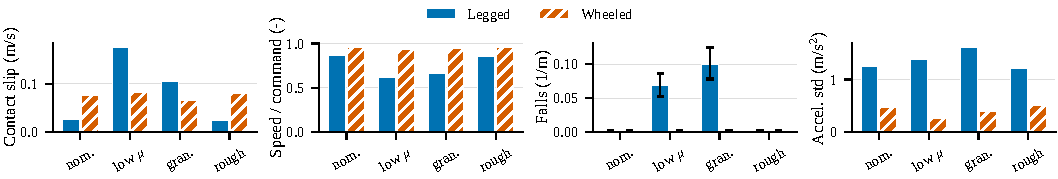
\includegraphics[width=\textwidth]{figures/fig2_configurations.pdf}
\caption{Dynamic behaviour by configuration and terrain, with 95\,\% credible intervals on falls. Wheeled slip and acceleration come from a different controller and contact geometry, and are not directly comparable with legged values.}
\label{fig:config}
\end{figure*}
\begin{figure*}[t]
\centering
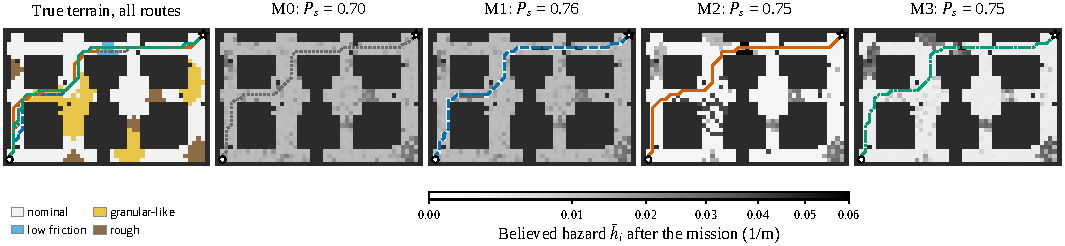
\includegraphics[width=\textwidth]{figures/fig4_risk_maps_trajectories.pdf}
\caption{One evaluation map (id 12, fixed in advance) at $\varepsilon=0.1$: true terrain with the four routes, and the hazard each method believes at mission end. Dots: start; stars: goal; dark cells: rock or high believed hazard. Here M1 happens to beat M2 and M3: the mean gain does not hold on every map.}
\label{fig:maps}
\end{figure*}

\emph{Monte Carlo.} Maps have $48\times32$ cells of 0.5\,m with drifts, crossings, rooms and pillars, and about \vhazFrac{}\,\% hazard coverage. Appearance is synthetic: per-map random prototypes with noise, so no terrain-to-look relation carries between maps; 15\,\% of hazard patches look like floor, and decoys make safe ground look hazardous. The Monte Carlo has no rendering, SLAM error or dynamics, and obstacles are known. Realised success draws one exponential threshold per replicate, shared across methods. Evaluation uses 200 maps with five replicates and common random numbers; the repetition uses 200 unseen maps. Parameters were tuned only on 50 development maps ($\sigma_k$=\vtunedKernelTwo{} for M2 and \vtunedKernelThree{} for M3, $\tau$=\vtunedTau{}, $\rho$=\vtunedRho{}, $\kappa$=\vtunedKappa{}; the last three at the edge of their grids). Fixed assumptions are $\lambda=25$, $\ell_w=1$\,m and hazard $[0.001,0.06,0.04,0.03]$\,m$^{-1}$ over $\mathcal{T}$, swept in Section~\ref{sec:sens}. In all, \vnMissionsTotal{} evaluation missions were run.

\emph{Statistics.} The map is the unit; replicates are averaged within it. We report 95\,\% bootstrap intervals of paired differences (10\,000 map resamples), Wilcoxon tests with Holm correction, and $d_z$. \sentbreak Hypotheses and refutation criteria were recorded before the campaigns: \textbf{H1} M2 beats M1 and M0; \textbf{H2} M1 beats M0; \textbf{H3} M3 beats M2; \textbf{H4} IMU plus joints beats each alone; \textbf{H5} the propagation gain differs between configurations through measured perception alone.

\section{Results and Discussion}
\subsection{Physical Behaviour}
The legged robot fell in \vfallsLegLow{} low-friction and \vfallsLegGran{} granular-like episodes and never on nominal or rough terrain, giving Jeffreys-posterior hazards of \vhLegLow{} and \vhLegGran{}\,m$^{-1}$, while contact slip rose from \vslipLegNom{} to \vslipLegLow{}\,m/s on low friction. The wheeled model never fell in 650 episodes, including ramps. The wheeled controller is ours, with a stiff stance, and has no fidelity claim, so the result describes these controllers only (Figs.~\ref{fig:mujoco} and~\ref{fig:config}).


\begin{figure*}[t]
\centering
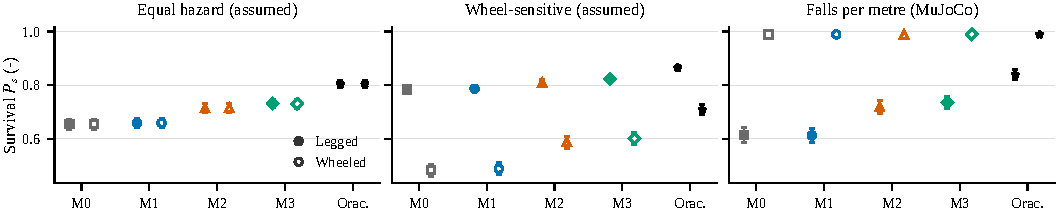
\includegraphics[width=\textwidth]{figures/fig3_measured_scenarios.pdf}
\caption{$P_s$ with measured classifier confusion (Fig.~\ref{fig:conf}) under three failure models (mean and 95\,\% interval, 200 maps). Filled: legged; open: wheeled. The configuration that gains most depends on the failure model.}
\label{fig:scen}
\end{figure*}
\begin{figure*}[t]
\centering
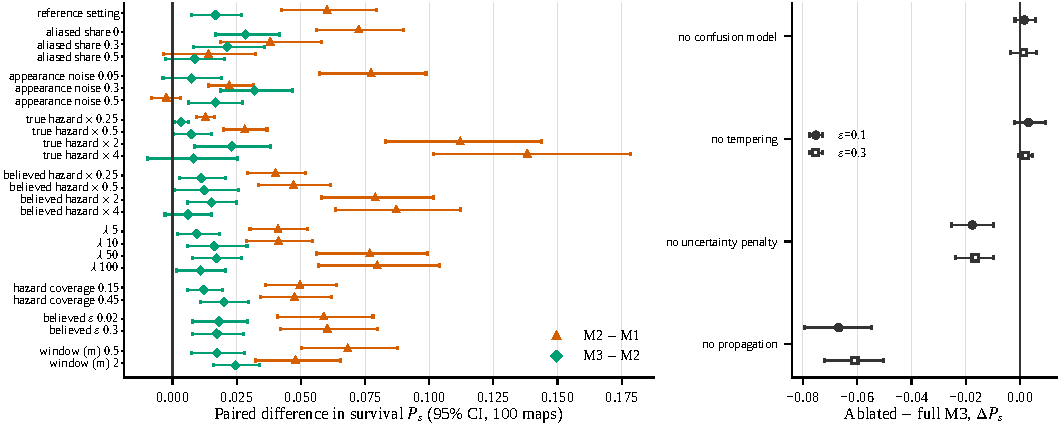
\includegraphics[width=\textwidth]{figures/fig8_sensitivity_ablation.pdf}
\caption{Left: sensitivity of the paired gains to assumed parameters at $\varepsilon=0.1$ (extremes of each sweep; the rest are in the repository). Right: ablation of M3 on 200 maps. Intervals crossing zero show no measurable effect.}
\label{fig:sens}
\end{figure*}

\subsection{Terrain Classification}
On \vnEpLeg{} legged and \vnEpWhe{} wheeled episodes (Table~\ref{tab:clf}), a random window split inflates legged macro-F1 from \vfOneLeg{} to \vfLeakLeg{}, which measures the leakage avoided. Held-out recall per class is \vrecLegNom{}, \vrecLegLow{}, \vrecLegGran{} and \vrecLegRough{} for nominal, low friction, granular-like and rough on the legged robot. Logistic regression does slightly better on the legged robot (\vfLogLeg{}, with lower calibration error); the forest stayed, as fixed in advance. H4 holds for the legged robot: fusion beats IMU by [\vfusImuLoLeg{}, \vfusImuHiLeg{}] and joints by [\vfusJointLoLeg{}, \vfusJointHiLeg{}]. For the wheeled robot the interval against IMU reaches zero, so H4 is not established there. The high scores say little about real ground: classes are separated by construction, and a wheeled F1 of \vfOneWhe{} mostly shows how clean simulated signals are. The stress tests are more informative. \sentbreak Mixed courses give \vfCourseLeg{} and \vfCourseWhe{}; with the legged robot, unseen speeds give as little as \vspeedLegMin{} (\vspeedLegLogMin{} with logistic regression) and unseen terrain parameters \vparamLegMin{}. Ramps, never trained on, are read as a hazard class in \vslopeHazardLeg{}\,\% (legged) and \vslopeHazardWhe{}\,\% (wheeled) of windows. The classifier interpolates within its training range and should not be trusted beyond it. Inference takes about \vinferMsLeg{}\,ms on a laptop core, not measured on the Jetson.

\begin{table}[!htb]
\centering
\caption{Classifier by Episode: Macro-F1 [95\,\% Interval] (Brier)}
\label{tab:clf}
\scriptsize
\resizebox{\columnwidth}{!}{\input{tables/tab_classifier.tex}}
\end{table}
\begin{figure}[!htb]
\centering
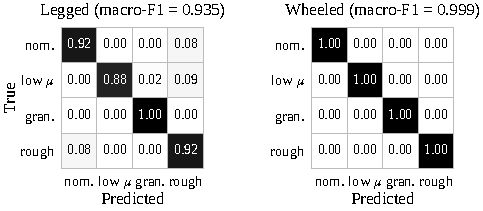
\includegraphics[width=\columnwidth]{figures/fig7_confusion.pdf}
\caption{Confusion on held-out episodes (fusion, forest), normalised by true class; source of the measured observation model.}
\label{fig:conf}
\end{figure}

\subsection{Map-Update Rules}
Tables~\ref{tab:main} and~\ref{tab:contrast} and Figs.~\ref{fig:maps} and~\ref{fig:robust} give the results. \textbf{H1 is supported}: at $\varepsilon=0.1$, M2 improves $P_s$ over M1 by \vdTwoOne{} [\vdTwoOneLo{}, \vdTwoOneHi{}], $d_z$=\vdTwoOneDz{}, and the repetition gives \vrepTwoOne{} [\vrepTwoOneLo{}, \vrepTwoOneHi{}]. Against M0, M2 and M3 cut the accumulated hazard by \vriskRedTwo{}\,\% and \vriskRedThree{}\,\%. The cost is \vlenAddTwo{}\,m of path and more replanning (\vrepMt{} against \vrepMo{} replans); a search took \vplanMsMt{}--\vplanMsMh{}\,ms on average in Python on a laptop. \textbf{H2 is not established}: M1 improves on M0 by only \vdOneZero{} [\vdOneZeroLo{}, \vdOneZeroHi{}], Holm-adjusted $p$=\vdOneZeroHolm{}, and the repetition interval [\vrepOneZeroLo{}, \vrepOneZeroHi{}] includes zero. Local updates arrive after the ground is crossed. \sentbreak A stronger baseline, added after internal review, also spreads evidence to cells within a 2\,m reach, by distance alone: it gains only \vspatialVsLocal{} [\vspatialVsLocalLo{}, \vspatialVsLocalHi{}] over M1, and M2 still beats it by \vspatialGain{} [\vspatialGainLo{}, \vspatialGainHi{}], so appearance, not mere spatial spread, carries the gain. \textbf{H3 is supported with a small effect}: M3 adds \vdThreeTwo{} [\vdThreeTwoLo{}, \vdThreeTwoHi{}] over M2, \vrepThreeTwo{} on repetition, growing with classifier error (\vdThreeTwoFive{} at $\varepsilon=0.5$). All methods stay well below the oracle bound of \vpsOrc{}.

\begin{table}[!htb]
\centering
\caption{Monte Carlo at $\varepsilon=0.1$, Equal Assumed Hazard (200 Maps, 95\,\% Bootstrap Intervals)}
\label{tab:main}
\scriptsize
\resizebox{\columnwidth}{!}{\input{tables/tab_main.tex}}
\end{table}
\begin{figure}[!htb]
\centering
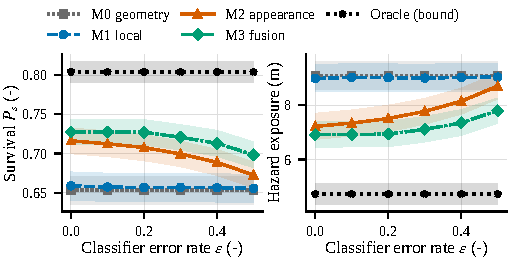
\includegraphics[width=\columnwidth]{figures/fig6_robustness.pdf}
\caption{Robustness to classifier error (mean and 95\,\% interval, 200 maps; synthetic symmetric confusion).}
\label{fig:robust}
\end{figure}
\begin{table}[!htb]
\centering
\caption{Paired Differences in $P_s$ [95\,\% Bootstrap Interval]}
\label{tab:contrast}
\scriptsize
\resizebox{\columnwidth}{!}{\input{tables/tab_contrasts.tex}}
\end{table}

\subsection{Does the Benefit Depend on the Feet?}
With equal assumed hazards and only the measured confusion differing, the M2$-$M1 gain is \vintLegEqual{} (legged) and \vintWheEqual{} (wheeled). \sentbreak Their difference, \vintDiffEqual{} [\vintLoEqual{}, \vintHiEqual{}], excludes zero, so H5 survives its recorded criterion, but the effect is negligible: perception quality creates no meaningful difference between configurations. Fig.~\ref{fig:scen} shows what does. With an assumed table that penalises wheels, the gain is larger for wheels (\vintWheSens{} against \vintLegSens{}). With simulated falls per metre (Fig.~\ref{fig:config}), the ordering reverses: legged \vintLegFalls{}, wheeled \vintWheFalls{}, because wheeled $P_s$ is already \vfallPsWheMz{} under M0, a level set by the Jeffreys prior since no fall occurred. An unmeasured table should therefore not be used to claim that one configuration benefits more. Mixed-course confusion lowers the M2 gain while M3 holds (Table~\ref{tab:contrast}).

\subsection{Sensitivity and Ablation}\label{sec:sens}
The propagation gain depends on the assumed appearance channel (Fig.~\ref{fig:sens}): it falls from \valiasZero{} with no aliasing to \valiasHigh{} [\valiasHighLo{}, \valiasHighHi{}] when half the patches are aliased, and to \vnoiseHigh{} [\vnoiseHighLo{}, \vnoiseHighHi{}] at high appearance noise. It scales with hazard, from \vhzLow{} to \vhzHigh{} across a 16-fold range. In M3, removing the confusion model (\vabConf{} [\vabConfLo{}, \vabConfHi{}]) or the tempering (\vabTemper{} [\vabTemperLo{}, \vabTemperHi{}]) has no measurable cost, so these are not supported as contributors. Removing propagation costs \vabProp{} and the uncertainty penalty \vabUnc{}. A higher $\lambda$ partly replaces that penalty, but even with each method at its best swept $\lambda$, M3 exceeds M2 by \vbestBest{} [\vbestBestLo{}, \vbestBestHi{}] at $\varepsilon=0.1$, so the soft fusion appears to account for the persistent part. This sweep is descriptive.

\subsection{Implications and Limitations}
Three points follow, conditional on this simulation. First, a local update alone arrives too late to change the route; its value is as a source of labels. Second, propagation is only as good as the appearance channel, so the first measurement to make is how well the robot's cameras separate physically different terrains. Third, failure must be measured for each configuration with its real controller before claiming that one benefits more.

No result comes from the physical robot, and none validates a real mine. The Monte Carlo is algorithmic: appearance is synthetic, so H1 rests on an assumption that vision must earn, and work on real images~\cite{wellhausen2019,mattamala2025} is the better guide to it. Falls are a narrow notion of failure. Joint signals have not been captured from the robot, and the sim-to-real gap of the classifier is unknown and likely large. Gazebo produced no result here, since it follows the pose computed by MuJoCo; under ROS~2 Jazzy its wheeled motion gate failed (0.184\,m/s after release).

\FloatBarrier
\section{Conclusion}
In this simulation study, spreading proprioceptive evidence by appearance raised mission survival, while updating only the crossed ground did almost nothing. A soft, uncertainty-penalised fusion added a small gain that grew with classifier error. The failure model, not perception, decided whether the benefit favours legs or wheels. Next steps are capturing joint signals on the robot under supervision, replacing synthetic appearance with camera features, and measuring failure on real surfaces.

\section*{Reproducibility}
Code, per-mission records with their seeds, evaluation maps, window features and the scripts that regenerate every number, table and figure are available at \url{https://github.com/JoseSegundoM/proprioceptive_risk_mapping}. The robot models come from the project repository \texttt{mine\_sentinel\_autonomy}, and raw MuJoCo signals are regenerated from their recorded seeds.

\interlinepenalty=10000  % a reference is never split across columns
\bibliographystyle{IEEEtran}
\bibliography{references}

\end{document}
.
% Requires \PaperTitle, \PaperAuthors (UTF-8, hyperref) and \PaperAuthorsPDF
% (PDFDocEncoding octal escapes, \pdfinfo) to be defined first.
\ifdefined\PDFPROFILE\else\def\PDFPROFILE{ieee}\fi
\def\profileinteractive{interactive}
\usepackage{tikz}
\usetikzlibrary{svg.path}
\definecolor{orcidlogocol}{HTML}{A6CE39}
% ORCID iD logo, same artwork as the orcidlink package (vector, no Type 3).
\newlength{\orcidxheight}
\newcommand{\orcidlogo}{\setlength{\orcidxheight}{\fontcharht\font`X}%
  \mbox{\begin{tikzpicture}[yscale=-0.00390625*\orcidxheight,
      xscale=0.00390625*\orcidxheight,transform shape]
    \fill[orcidlogocol] svg{M256,128c0,70.7-57.3,128-128,128C57.3,256,0,198.7,0,128C0,57.3,57.3,0,128,0C198.7,0,256,57.3,256,128z};
    \fill[white] svg{M86.3,186.2H70.9V79.1h15.4v48.4V186.2z}
      svg{M108.9,79.1h41.6c39.6,0,57,28.3,57,53.6c0,27.5-21.5,53.6-56.8,53.6h-41.8V79.1z M124.3,172.4h24.5c34.9,0,42.9-26.5,42.9-39.7c0-21.5-13.7-39.7-43.7-39.7h-23.7V172.4z}
      svg{M88.7,56.8c0,5.5-4.5,10.1-10.1,10.1c-5.6,0-10.1-4.6-10.1-10.1c0-5.6,4.5-10.1,10.1-10.1C84.2,46.7,88.7,51.3,88.7,56.8z};
  \end{tikzpicture}}}
\ifx\PDFPROFILE\profileinteractive
  \usepackage[colorlinks=true,linkcolor=black,citecolor=black,urlcolor=blue,
              bookmarks=false]{hyperref}
  \hypersetup{pdftitle={\PaperTitle},pdfauthor={\PaperAuthors}}
  \newcommand{\orcid}[1]{\href{https://orcid.org/#1}{\orcidlogo}}
  \newcommand{\authoremail}[1]{\href{mailto:#1}{#1}}
  \newcommand{\doititle}[2]{\href{https://doi.org/#1}{#2}}
  \newcommand{\urltitle}[2]{\href{#1}{#2}}
\else
  \pdfinfo{/Title (\PaperTitle) /Author (\PaperAuthorsPDF)}
  \newcommand{\orcid}[1]{\orcidlogo}
  \newcommand{\authoremail}[1]{#1}
  \newcommand{\doititle}[2]{#2}
  \newcommand{\urltitle}[2]{#2}
\fi

\usetikzlibrary{arrows.meta,backgrounds,fit,calc}
\definecolor{amberfill}{HTML}{FBEFC9}
\definecolor{greenfill}{HTML}{E3F1EC}
\urlstyle{same}
\newcommand{\vabConf}{+0.002}
\newcommand{\vabConfHi}{+0.006}
\newcommand{\vabConfLo}{\mbox{$-$}0.002}
\newcommand{\vabProp}{\mbox{$-$}0.067}
\newcommand{\vabPropHi}{\mbox{$-$}0.055}
\newcommand{\vabPropLo}{\mbox{$-$}0.080}
\newcommand{\vabTemper}{+0.003}
\newcommand{\vabTemperHi}{+0.009}
\newcommand{\vabTemperLo}{\mbox{$-$}0.002}
\newcommand{\vabUnc}{\mbox{$-$}0.018}
\newcommand{\vabUncHi}{\mbox{$-$}0.010}
\newcommand{\vabUncLo}{\mbox{$-$}0.025}
\newcommand{\valiasHigh}{+0.014}
\newcommand{\valiasHighHi}{+0.032}
\newcommand{\valiasHighLo}{\mbox{$-$}0.003}
\newcommand{\valiasZero}{+0.072}
\newcommand{\vbestBest}{+0.013}
\newcommand{\vbestBestHi}{+0.021}
\newcommand{\vbestBestLo}{+0.005}
\newcommand{\vdOneZero}{+0.004}
\newcommand{\vdOneZeroDz}{0.15}
\newcommand{\vdOneZeroHi}{+0.007}
\newcommand{\vdOneZeroHolm}{0.055}
\newcommand{\vdOneZeroLo}{+0.000}
\newcommand{\vdThreeOne}{+0.070}
\newcommand{\vdThreeOneDz}{0.74}
\newcommand{\vdThreeOneHi}{+0.084}
\newcommand{\vdThreeOneHolm}{0.000}
\newcommand{\vdThreeOneLo}{+0.057}
\newcommand{\vdThreeTwo}{+0.015}
\newcommand{\vdThreeTwoDz}{0.28}
\newcommand{\vdThreeTwoFive}{+0.026}
\newcommand{\vdThreeTwoFiveDz}{0.49}
\newcommand{\vdThreeTwoFiveHi}{+0.033}
\newcommand{\vdThreeTwoFiveHolm}{0.000}
\newcommand{\vdThreeTwoFiveLo}{+0.019}
\newcommand{\vdThreeTwoHi}{+0.023}
\newcommand{\vdThreeTwoHolm}{0.000}
\newcommand{\vdThreeTwoLo}{+0.008}
\newcommand{\vdThreeZero}{+0.074}
\newcommand{\vdThreeZeroDz}{0.77}
\newcommand{\vdThreeZeroHi}{+0.088}
\newcommand{\vdThreeZeroHolm}{0.000}
\newcommand{\vdThreeZeroLo}{+0.061}
\newcommand{\vdTwoOne}{+0.055}
\newcommand{\vdTwoOneDz}{0.64}
\newcommand{\vdTwoOneFive}{+0.017}
\newcommand{\vdTwoOneFiveDz}{0.22}
\newcommand{\vdTwoOneFiveHi}{+0.028}
\newcommand{\vdTwoOneFiveHolm}{0.019}
\newcommand{\vdTwoOneFiveLo}{+0.007}
\newcommand{\vdTwoOneHi}{+0.067}
\newcommand{\vdTwoOneHolm}{0.000}
\newcommand{\vdTwoOneLo}{+0.043}
\newcommand{\vdTwoZero}{+0.059}
\newcommand{\vdTwoZeroDz}{0.67}
\newcommand{\vdTwoZeroHi}{+0.071}
\newcommand{\vdTwoZeroHolm}{0.000}
\newcommand{\vdTwoZeroLo}{+0.047}
\newcommand{\vexpMh}{6.92}
\newcommand{\vexpMo}{9.03}
\newcommand{\vexpMt}{7.35}
\newcommand{\vexpMz}{9.10}
\newcommand{\vexpOrc}{4.73}
\newcommand{\vexpRedTwoAbs}{1.75}
\newcommand{\vfCourseLeg}{0.820}
\newcommand{\vfCourseWhe}{0.842}
\newcommand{\vfHeldLeg}{0.935}
\newcommand{\vfHeldWhe}{0.999}
\newcommand{\vfLeakLeg}{0.982}
\newcommand{\vfLeakWhe}{0.999}
\newcommand{\vfOneLeg}{0.956}
\newcommand{\vfOneWhe}{0.998}
\newcommand{\vfallOneZero}{\mbox{$-$}0.002}
\newcommand{\vfallOneZeroDz}{\mbox{$-$}0.07}
\newcommand{\vfallOneZeroHi}{+0.002}
\newcommand{\vfallOneZeroHolm}{0.362}
\newcommand{\vfallOneZeroLo}{\mbox{$-$}0.007}
\newcommand{\vfallPsLegMh}{0.734}
\newcommand{\vfallPsLegMz}{0.614}
\newcommand{\vfallPsLegOrc}{0.840}
\newcommand{\vfallPsWheMh}{0.989}
\newcommand{\vfallPsWheMz}{0.989}
\newcommand{\vfallPsWheOrc}{0.989}
\newcommand{\vfallThreeTwo}{+0.016}
\newcommand{\vfallThreeTwoDz}{0.16}
\newcommand{\vfallThreeTwoHi}{+0.030}
\newcommand{\vfallThreeTwoHolm}{0.002}
\newcommand{\vfallThreeTwoLo}{+0.003}
\newcommand{\vfallTwoOne}{+0.106}
\newcommand{\vfallTwoOneDz}{0.71}
\newcommand{\vfallTwoOneHi}{+0.127}
\newcommand{\vfallTwoOneHolm}{0.000}
\newcommand{\vfallTwoOneLo}{+0.086}
\newcommand{\vfallsLegGran}{70/150}
\newcommand{\vfallsLegLow}{61/150}
\newcommand{\vfallsLegNom}{0/150}
\newcommand{\vfallsLegRough}{0/150}
\newcommand{\vfallsWheGran}{0/150}
\newcommand{\vfallsWheLow}{0/150}
\newcommand{\vfallsWheNom}{0/150}
\newcommand{\vfallsWheRough}{0/150}
\newcommand{\vfusImuHiLeg}{+0.0248}
\newcommand{\vfusImuHiWhe}{+0.0036}
\newcommand{\vfusImuLoLeg}{+0.0100}
\newcommand{\vfusImuLoWhe}{\mbox{$-$}0.0000}
\newcommand{\vfusJointHiLeg}{+0.057}
\newcommand{\vfusJointHiWhe}{+0.011}
\newcommand{\vfusJointLoLeg}{+0.033}
\newcommand{\vfusJointLoWhe}{+0.006}
\newcommand{\vhLegGran}{0.100}
\newcommand{\vhLegLow}{0.068}
\newcommand{\vhLegNom}{0.000}
\newcommand{\vhLegRough}{0.000}
\newcommand{\vhWheGran}{0.000}
\newcommand{\vhWheLow}{0.000}
\newcommand{\vhWheNom}{0.000}
\newcommand{\vhWheRough}{0.000}
\newcommand{\vhazFrac}{31}
\newcommand{\vhzHigh}{+0.138}
\newcommand{\vhzLow}{+0.013}
\newcommand{\vinferMsLeg}{10}
\newcommand{\vinferMsWhe}{10}
\newcommand{\vintDiffEqual}{+0.002}
\newcommand{\vintDiffFalls}{\mbox{$-$}0.106}
\newcommand{\vintDiffSens}{+0.075}
\newcommand{\vintHiEqual}{+0.004}
\newcommand{\vintHiFalls}{\mbox{$-$}0.086}
\newcommand{\vintHiSens}{+0.091}
\newcommand{\vintLegEqual}{+0.055}
\newcommand{\vintLegFalls}{+0.106}
\newcommand{\vintLegSens}{+0.023}
\newcommand{\vintLoEqual}{+0.001}
\newcommand{\vintLoFalls}{\mbox{$-$}0.127}
\newcommand{\vintLoSens}{+0.060}
\newcommand{\vintWheEqual}{+0.057}
\newcommand{\vintWheFalls}{+0.000}
\newcommand{\vintWheSens}{+0.098}
\newcommand{\vlamHighNouncThree}{0.744}
\newcommand{\vlamHighThree}{0.743}
\newcommand{\vlamHighTwo}{0.728}
\newcommand{\vlenAddThree}{0.35}
\newcommand{\vlenAddTwo}{0.37}
\newcommand{\vlenMh}{33.0}
\newcommand{\vlenMo}{32.6}
\newcommand{\vlenMt}{33.0}
\newcommand{\vlenMz}{32.6}
\newcommand{\vlenOrc}{33.4}
\newcommand{\vnCourseLeg}{49}
\newcommand{\vnCourseWhe}{50}
\newcommand{\vnEpLeg}{495}
\newcommand{\vnEpWhe}{600}
\newcommand{\vnEpisodesTotal}{1400}
\newcommand{\vnMissionsTotal}{177\,000}
\newcommand{\vnWinLeg}{6206}
\newcommand{\vnWinWhe}{7800}
\newcommand{\vnoiseHigh}{\mbox{$-$}0.002}
\newcommand{\vnoiseHighHi}{+0.003}
\newcommand{\vnoiseHighLo}{\mbox{$-$}0.008}
\newcommand{\vparamLegMin}{0.696}
\newcommand{\vplanMsMh}{4.0}
\newcommand{\vplanMsMo}{4.4}
\newcommand{\vplanMsMt}{3.3}
\newcommand{\vplanMsMz}{10.4}
\newcommand{\vplanMsOrc}{7.9}
\newcommand{\vpsFiveMh}{0.698}
\newcommand{\vpsFiveMo}{0.656}
\newcommand{\vpsFiveMt}{0.672}
\newcommand{\vpsFiveMz}{0.654}
\newcommand{\vpsFiveOrc}{0.804}
\newcommand{\vpsMh}{0.727}
\newcommand{\vpsMo}{0.657}
\newcommand{\vpsMt}{0.712}
\newcommand{\vpsMz}{0.654}
\newcommand{\vpsOrc}{0.804}
\newcommand{\vrepFallTwoOne}{+0.075}
\newcommand{\vrepFallTwoOneDz}{0.58}
\newcommand{\vrepFallTwoOneHi}{+0.093}
\newcommand{\vrepFallTwoOneHolm}{0.000}
\newcommand{\vrepFallTwoOneLo}{+0.057}
\newcommand{\vrepMh}{12.1}
\newcommand{\vrepMo}{4.5}
\newcommand{\vrepMt}{19.5}
\newcommand{\vrepMz}{0.0}
\newcommand{\vrepOneZero}{+0.001}
\newcommand{\vrepOneZeroDz}{0.05}
\newcommand{\vrepOneZeroHi}{+0.004}
\newcommand{\vrepOneZeroHolm}{0.044}
\newcommand{\vrepOneZeroLo}{\mbox{$-$}0.002}
\newcommand{\vrepOrc}{0.0}
\newcommand{\vrepThreeTwo}{+0.014}
\newcommand{\vrepThreeTwoDz}{0.35}
\newcommand{\vrepThreeTwoHi}{+0.019}
\newcommand{\vrepThreeTwoHolm}{0.000}
\newcommand{\vrepThreeTwoLo}{+0.008}
\newcommand{\vrepTwoOne}{+0.049}
\newcommand{\vrepTwoOneDz}{0.62}
\newcommand{\vrepTwoOneHi}{+0.059}
\newcommand{\vrepTwoOneHolm}{0.000}
\newcommand{\vrepTwoOneLo}{+0.038}
\newcommand{\vriskRedOne}{1.3}
\newcommand{\vriskRedThree}{26}
\newcommand{\vriskRedTwo}{21}
\newcommand{\vslipLegGran}{0.105}
\newcommand{\vslipLegLow}{0.175}
\newcommand{\vslipLegNom}{0.027}
\newcommand{\vslipLegRough}{0.025}
\newcommand{\vslipWheGran}{0.065}
\newcommand{\vslipWheLow}{0.082}
\newcommand{\vslipWheNom}{0.076}
\newcommand{\vslipWheRough}{0.080}
\newcommand{\vslopeHazardLeg}{99}
\newcommand{\vslopeHazardWhe}{79}
\newcommand{\vslopeNomLeg}{1}
\newcommand{\vslopeNomWhe}{21}
\newcommand{\vspatialGain}{+0.053}
\newcommand{\vspatialGainHi}{+0.065}
\newcommand{\vspatialGainLo}{+0.042}
\newcommand{\vspatialVsLocal}{+0.002}
\newcommand{\vspatialVsLocalHi}{+0.006}
\newcommand{\vspatialVsLocalLo}{\mbox{$-$}0.002}
\newcommand{\vspeedLegLogMin}{0.658}
\newcommand{\vspeedLegMin}{0.450}
\newcommand{\vsuccZeroMh}{0.735}
\newcommand{\vsuccZeroMo}{0.670}
\newcommand{\vsuccZeroMt}{0.710}
\newcommand{\vsuccZeroMz}{0.665}
\newcommand{\vsuccZeroOrc}{0.815}
\newcommand{\vtrackLegGran}{0.66}
\newcommand{\vtrackLegLow}{0.62}
\newcommand{\vtrackLegNom}{0.87}
\newcommand{\vtrackLegRough}{0.85}
\newcommand{\vtrackWheGran}{0.95}
\newcommand{\vtrackWheLow}{0.93}
\newcommand{\vtrackWheNom}{0.96}
\newcommand{\vtrackWheRough}{0.95}
\newcommand{\vtunedKappa}{1}
\newcommand{\vtunedKernelThree}{0.5}
\newcommand{\vtunedKernelTwo}{0.35}
\newcommand{\vtunedRho}{0.6}
\newcommand{\vtunedTau}{0.5}
\newcommand{\vwheelShiftMin}{0.935}
\newcommand{\vwilsonHiMh}{0.791}
\newcommand{\vwilsonHiMo}{0.731}
\newcommand{\vwilsonHiMt}{0.768}
\newcommand{\vwilsonHiMz}{0.727}
\newcommand{\vwilsonHiOrc}{0.863}
\newcommand{\vwilsonLoMh}{0.670}
\newcommand{\vwilsonLoMo}{0.602}
\newcommand{\vwilsonLoMt}{0.644}
\newcommand{\vwilsonLoMz}{0.597}
\newcommand{\vwilsonLoOrc}{0.755}

\renewcommand{\topfraction}{0.92}
\renewcommand{\bottomfraction}{0.85}
\renewcommand{\textfraction}{0.07}
\renewcommand{\floatpagefraction}{0.80}
\setlength{\textfloatsep}{7pt plus 2pt minus 2pt}
\setlength{\floatsep}{7pt plus 2pt minus 2pt}
\setlength{\intextsep}{7pt plus 2pt minus 2pt}
\setlength{\abovecaptionskip}{3pt}
\setlength{\belowcaptionskip}{0pt}

\clubpenalty=10000
\widowpenalty=10000
\displaywidowpenalty=10000
\newcommand{\sentbreak}{\par\pagebreak\noindent}  % a column ends only at the end of a sentence (scripts/fix_breaks.py)

% Fixed heading space: a column that ends early spreads its gap over all its lines, a fraction of a point each.
\makeatletter
\def\section{\@startsection{section}{1}{\z@}{1.5ex}{0.7ex}{\normalfont\normalsize\centering\scshape}}
\def\subsection{\@startsection{subsection}{2}{\z@}{1.2ex}{0.5ex}{\normalfont\normalsize\itshape}}
\makeatother
\setlength{\parskip}{0pt}
\flushbottom
\AtBeginDocument{\setlength{\baselineskip}{12pt plus 0.8pt}}

\begin{document}

\title{Proprioception-Augmented Risk Mapping for a Commercial Quadruped: Terrain-Aware Navigation Across Legged and Wheeled Configurations}

\author{\IEEEauthorblockN{Jose Luis Segundo Manayay\,\orcid{0009-0002-9203-8710},
Javier Yanpier Garay Yovera\,\orcid{0009-0001-1645-8724},
Francisco Jes\'us Rodr\'iguez Huiman\,\orcid{0009-0006-6972-2484}}
\IEEEauthorblockA{Universidad Nacional de Ingenier\'ia (UNI), Faculty of Mechanical Engineering, Lima, Peru\\
\authoremail{jose.segundo.m@uni.pe}; \authoremail{javier.garay.y@uni.pe}; \authoremail{francisco.rodriguez.h@uni.pe}}}

\maketitle

\begin{abstract}
Inspection robots build risk maps from geometry, yet slippery or soft ground can look as flat as concrete. This paper studies how proprioceptive evidence should enter a risk map, and whether its value depends on the foot configuration of a commercial quadruped, the DOBOT Rover X1, whose legged and wheeled configurations are fixed before a mission. In MuJoCo, \vnEpisodesTotal{} dynamic episodes on parametrised terrain train a lightweight classifier and measure falls per metre. A separate Monte Carlo study compares geometry-only mapping, local Bayesian updating, appearance-based propagation and an uncertainty-aware fusion on 200 procedural indoor maps with paired statistics. Propagation raised mission survival probability by 0.055 over local updating and fusion added 0.015; both effects held on 200 independent maps, while local updating was practically indistinguishable from geometry. In simulation the legged robot fell on low-friction and soft terrain and the wheeled model never fell, so the benefit of propagation followed the failure model, not perception quality. The classifier reached macro-F1 of 0.935 and 0.999 on held-out episodes but dropped to 0.45 for the legged robot at unseen speeds. All results are simulation only; appearance features remain assumed and no hardware validation is claimed.
\end{abstract}

\begin{IEEEkeywords}
legged robots, wheeled-legged robots, proprioception, terrain classification, traversability, risk-aware planning, Monte Carlo simulation
\end{IEEEkeywords}

\section{Introduction}
Autonomous inspection of underground and industrial spaces depends on knowing which ground can be crossed. Quadrupeds have operated in such settings~\cite{tranzatto2022,gao2026}, but geometry says little about friction or softness: a wet floor and dry concrete return the same LiDAR profile, and the robot learns the difference only on contact. Commercial quadrupeds expose joint and inertial signals that could reveal it, behind closed locomotion controllers.

This raises a question separate from the classifier itself: \emph{how should a proprioceptive detection enter the planner's risk map?} It can update only the ground already crossed, or generalise to unvisited ground that looks alike. A second question is whether the answer depends on the feet. The DOBOT Rover X1 uses point-foot and wheel modules that are exchanged by hand (Fig.~\ref{fig:quadrupeds}), so the configuration is fixed before a mission; we treat them as two robots and model no switching.

\begin{figure}[!t]
\centering
\ifdefined\REALPHOTOS
{\scriptsize\setlength{\tabcolsep}{1.5pt}\begin{tabular}{cc}
(a) Legged & (b) Wheeled\\
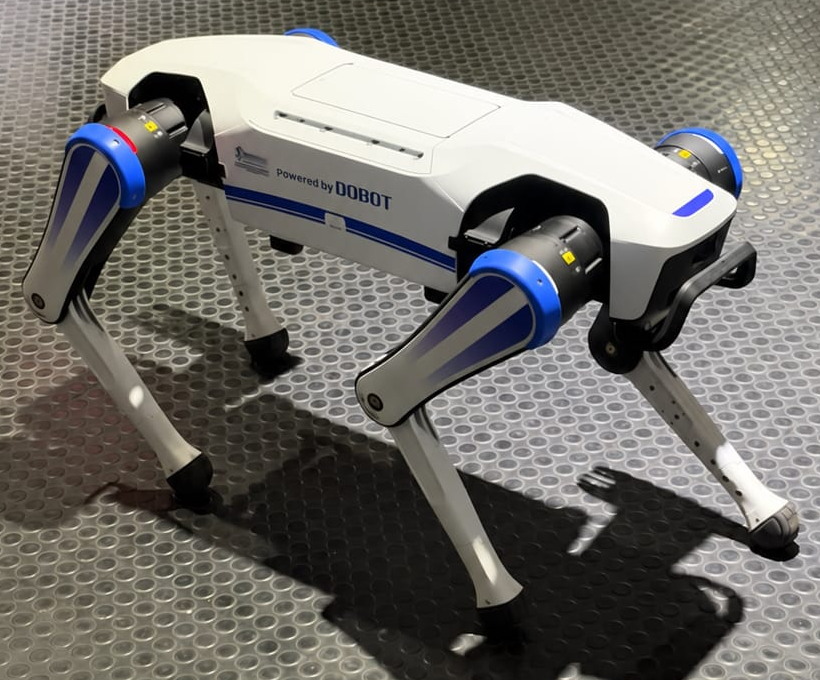
\includegraphics[height=28mm]{figures/photos/robot_legged.png} & 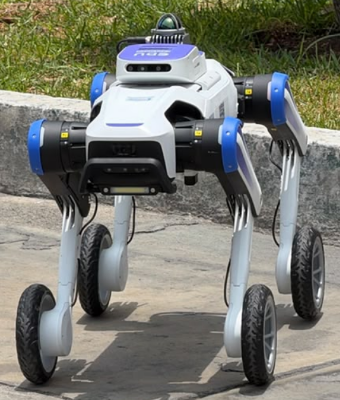
\includegraphics[height=28mm]{figures/photos/robot_wheeled.png}
\end{tabular}}
\caption{The physical DOBOT Rover X1: (a) legged, with point feet; (b) wheeled, with wheel modules. The modules are exchanged by hand, so each mission uses one configuration. The results of this paper come from simulation, not from these scenes.}
\else
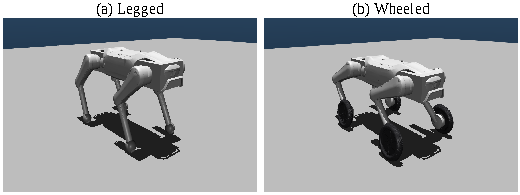
\includegraphics[width=\columnwidth]{figures/fig0_quadrupeds.pdf}
\caption{The two configurations studied, as MuJoCo simulation renders, not photographs: (a) legged, with point feet and 12 actuators; (b) wheeled, with wheel modules and 16 actuators. On the robot the modules are exchanged by hand, so each mission uses one configuration.}
\fi
\label{fig:quadrupeds}
\end{figure}

Comparisons of this kind risk circularity: if failure rates are assumed to differ between wheels and legs, finding that the benefit differs restates the assumption. \sentbreak We therefore separate perception from failure and measure both in dynamic simulation where possible. Our contributions are:
\begin{enumerate}
\item A reproducible, paired Monte Carlo comparison of four map-update rules, with independent repetition and sensitivity analysis.
\item A dynamic-simulation dataset of both configurations on parametrised terrain, and a lightweight classifier stress-tested beyond its training range.
\item Evidence that the failure model decides how the benefit depends on the feet: simulated falls reverse which configuration gains.
\end{enumerate}
This work follows our inspection architecture on a small servo-driven platform~\cite{segundo2026laccei}, but addresses a different question on a different robot. We claim no novelty for the fusion rule, a tempered Bayesian update of known form~\cite{bissiri2016}.

\begin{figure*}[t]
\centering
\resizebox{\textwidth}{!}{% Study structure. Colour = status of each block.
\begin{tikzpicture}[font=\scriptsize,>={Latex[length=1.6mm]},line width=0.45pt,
  box/.style={draw,rounded corners=1.2pt,align=center,text width=29mm,minimum height=11mm,inner sep=1.5pt,fill=white},
  assumed/.style={box,fill=amberfill},
  new/.style={box,fill=greenfill},
  lab/.style={font=\scriptsize\bfseries,inner sep=0pt},
  note/.style={font=\tiny,inner sep=0.8pt,fill=white}]
\def\xa{1.6}\def\xb{5.0}\def\xc{8.4}\def\xd{11.8}\def\xe{15.2}
% Lanes
\fill[black!4,draw=black!40,rounded corners=2pt] (-0.05,2.25) rectangle (16.85,4.05);
\fill[black!4,draw=black!40,rounded corners=2pt] (-0.05,-0.95) rectangle (16.85,1.0);
\node[lab,anchor=north west] at (0.08,3.97) {Dynamic simulation (MuJoCo): measured in simulation};
\node[lab,anchor=south west] at (0.08,-0.88) {Algorithmic Monte Carlo: no dynamics, no rendering};
% Dynamic simulation
\node[assumed] (terrain) at (\xa,2.9) {Terrain parameters\\friction, relief, contact\\(assumed ranges)};
\node[box]     (robot)   at (\xb,2.9) {Robot models, controllers\\legged: maker's policy\\wheeled: project's own};
\node[new]     (signals) at (\xc,2.9) {Proprioception\\IMU, joint position,\\velocity, command torque};
\node[new]     (clf)     at (\xd,2.9) {Terrain classifier\\window features,\\random forest};
\node[new]     (conf)    at (\xe,2.9) {Held-out confusion\\$\hat p(o\mid t,c)$,\\split by episode};
\draw[->] (terrain)--(robot); \draw[->] (robot)--(signals); \draw[->] (signals)--(clf); \draw[->] (clf)--(conf);
% Monte Carlo
\node[assumed] (maps) at (\xa,0.28) {Procedural maps\\geometry and synthetic\\appearance};
\node[new]     (bel)  at (\xb,0.28) {Belief update\\M0 geometry, M1 local,\\M2 vote, M3 fusion};
\node[new]     (plan) at (\xc,0.28) {Risk-aware A*\\rate $1+\lambda(\bar h_i+\kappa\sigma_i)$\\replanning};
\node[new]     (mis)  at (\xd,0.28) {Mission\\true hazard accumulates,\\hidden from the methods};
\node[new]     (out)  at (\xe,0.28) {Paired statistics\\$P_s$, exposure, length,\\by map};
\draw[->] (maps)--(bel); \draw[->] (bel)--(plan); \draw[->] (plan)--(mis); \draw[->] (mis)--(out);
\draw[->,dashed] (mis.south) -- (\xd,-0.58) -- (\xb,-0.58) -- (bel.south);
\node[note,fill=black!4] at (8.4,-0.58) {new window $(o,c)$, then replan};
% Offline bridges
\draw[->,line width=0.8pt] ([xshift=-7mm]robot.south) -- ([xshift=-7mm]robot.south |- 0,1.62) -- ([xshift=-6mm]mis.north |- 0,1.62) -- ([xshift=-6mm]mis.north);
\node[note] at (7.6,1.62) {falls per metre, one of the failure models (offline)};
\draw[->,line width=0.8pt] (conf.south) -- (\xe,1.62) -- ([xshift=6mm]mis.north |- 0,1.62) -- ([xshift=6mm]mis.north);
\node[note] at (14.25,1.62) {observation model (offline)};
% Legend
\node[draw,fill=amberfill,minimum width=3mm,minimum height=2mm,inner sep=0,label={[font=\tiny,inner sep=1pt]right:assumed}] at (9.15,3.82) {};
\node[draw,fill=greenfill,minimum width=3mm,minimum height=2mm,inner sep=0,label={[font=\tiny,inner sep=1pt]right:implemented here}] at (10.75,3.82) {};
\node[draw,fill=white,minimum width=3mm,minimum height=2mm,inner sep=0,label={[font=\tiny,inner sep=1pt]right:from the manufacturer or the project}] at (13.0,3.82) {};
\end{tikzpicture}
}
\caption{Study structure. Dynamic simulation supplies the classifier, its held-out confusion and fall rates; these enter the algorithmic Monte Carlo offline, where each method sees only its own observations. Colour gives the status of each block.}
\label{fig:arch}
\end{figure*}

\section{Related Work}
Wheels on a quadruped can greatly reduce the cost of transport~\cite{bjelonic2019}, and learned controllers achieve robust hybrid navigation~\cite{lee2024}, but those systems own their controller; here perception and planning act above a closed one. Terrain can be classified from foot forces and joint signals~\cite{bednarek2019}, soils inspected haptically~\cite{kolvenbach2019}, compliance estimated online for control~\cite{fahmi2020}, and traversability estimated from legged proprioception~\cite{elnoor2024}. We ask instead how such an estimate should spread through a map. Self-supervised methods project proprioceptive labels onto images~\cite{wellhausen2019}, Wild Visual Navigation learns traversability online from visual features~\cite{mattamala2025}, and terrain-property maps combine semantics with proprioceptive estimates~\cite{ewen2022}. Those works use real robots and images, which we do not. \sentbreak Our addition is narrower: a paired measurement of what propagation is worth as classification error and appearance ambiguity vary. Risk-aware planners use CVaR over traversability~\cite{fan2021} or evidential uncertainty~\cite{cai2024}; our simpler planner is only a common testbed.

\begin{figure*}[t]
\centering
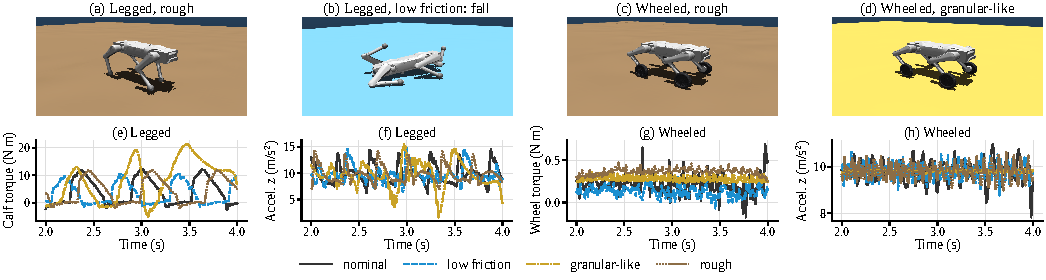
\includegraphics[width=\textwidth]{figures/fig9_mujoco.pdf}
\caption{MuJoCo simulation. (a)--(d) Renders of campaign episodes, with floor colour added for display only. (e)--(h) Logged signals over 2\,s on the four terrains, from example episodes that lasted at least 5.5\,s. Commanded torque is the actuator command, not a contact force.}
\label{fig:mujoco}
\end{figure*}
\section{Platform and Simulation Models}
The manufacturer specifies 15.5\,kg with point feet and 18.5\,kg with wheels, a Livox Mid-360 LiDAR, a RealSense D435i and a Jetson Orin Nano. Dynamics use MuJoCo~\cite{todorov2012} with models built from the manufacturer's files (the study is outlined in Fig.~\ref{fig:arch} and its control structure in Fig.~\ref{fig:control}). The legged model has 12 actuators and walks on the manufacturer's trained policy; the wheeled model has 16 and rolls on a skid-steer controller written for the project, because the manufacturer's is not public. The models weigh 18.65 and 22.08\,kg, not rescaled because the source of the difference is unknown. They are not calibrated digital twins.

Validating the models changed the setup. At the project's 200\,Hz control rate, the wheeled stance PD (400\,N\,m/rad, 7\,N\,m\,s/rad) produced a numerical limit cycle of about 70\,m/s$^2$ RMS at the IMU, even on a plane, which a classifier would learn as an artefact. We run physics and the stance PD at 1\,kHz, as a joint servo would; mean vertical contact force then matches model weight within 1\,\% on nominal terrain. The floor has contact priority, since MuJoCo otherwise uses the larger friction of a pair.

\begin{figure}[t]
\centering
\resizebox{\columnwidth}{!}{% Control structure: inner loop in MuJoCo, outer loop in the Monte Carlo, joined offline.
\begin{tikzpicture}[font=\scriptsize,>={Latex[length=1.5mm]},line width=0.45pt,
  block/.style={draw,rounded corners=0.8pt,align=center,minimum height=8.5mm,inner sep=1.5pt,fill=white},
  sum/.style={draw,circle,inner sep=0,minimum size=3.2mm,fill=white},
  sig/.style={font=\tiny,inner sep=0.8pt}]
\fill[black!4,draw=black!50,dashed,rounded corners=2pt] (2.0,0.72) rectangle (9.3,3.0);
\node[font=\tiny\bfseries,anchor=north east,inner sep=1pt] at (9.22,2.95) {Inner loop: MuJoCo};
% outer, top row
\node[block,fill=greenfill,text width=15mm] (risk) at (0.75,3.95) {Risk map\\$\bar h_i,\ \sigma_i$};
\node[block,fill=greenfill,text width=15mm] (astar) at (3.25,3.95) {A* planner\\min $J$};
\draw[->] (risk) -- node[sig,above] {cost} (astar);
\node[font=\tiny,align=left,anchor=west,inner sep=0pt] at (4.2,3.95) {\textbf{Outer loop: Monte Carlo}\\through the belief update;\\the dashed link is offline};
% inner, middle row
\node[block,text width=15mm] (ctl) at (3.25,1.95) {Locomotion\\policy, 50\,Hz\\or skid-steer};
\node[sum] (s) at (5.0,1.95) {};
\node[block,text width=9mm] (pd) at (6.05,1.95) {Joint\\PD};
\node[block,text width=13mm] (rob) at (7.9,1.95) {Robot and\\terrain\\contact};
\draw[->] (astar) -- node[sig,right,pos=0.28,align=left] {$v_x,\omega_z$} (ctl);
\draw[->] (ctl) -- node[sig,above] {$q_d$} (s);
\draw[->] (s) -- (pd);
\draw[->] (pd) -- node[sig,above] {$\tau$} (rob);
\coordinate (out) at (9.0,1.95);
\draw (rob) -- (out);
\node[sig,above] at (8.9,1.97) {$y$};
% feedback
\draw[->] (out) -- (9.0,1.02) -- (5.0,1.02) -- (s.south);
\node[sig,anchor=east] at (4.92,1.5) {$-$};
\node[sig,above] at (7.0,1.02) {$q,\dot q$};
\draw[->] (5.0,1.02) -- (3.25,1.02) -- (ctl.south);
\node[sig,above] at (4.15,1.02) {$q,\dot q$, IMU};
\fill (5.0,1.02) circle (0.5pt);
% outer, bottom row
\node[block,fill=greenfill,text width=16mm] (clf) at (7.9,0.0) {Features and\\classifier};
\node[block,fill=greenfill,text width=15mm] (bel) at (0.75,0.0) {Belief update\\M0--M3};
\draw[->,dashed] (9.0,1.02) -- (9.0,0.0) -- (clf.east);
\draw[->] (clf) -- node[sig,above] {class $o$, confidence $c$} (bel);
\draw[->] (bel) -- node[sig,right,align=left] {$b_i(t)$} (risk);
\end{tikzpicture}
}
\caption{Control structure. The inner loop runs in MuJoCo; $y$ is the proprioceptive output. The outer loop runs in the Monte Carlo and is joined to the inner loop offline (dashed), through the classifier's confusion. The two were not closed online in one simulator.}
\label{fig:control}
\end{figure}

\section{Method}
\emph{Hazard.} A mission crosses terrain of true class $t_k\in\mathcal{T}=\{$nominal, low friction, granular-like, rough$\}$ over segments $\ell_k$. With per-metre hazard $h(t)$ and a patch multiplier $m_k$, survival is
\begin{equation}
P_s=\exp(-H),\qquad H=\sum_k \ell_k\, m_k\, h(t_k),
\label{eq:survival}
\end{equation}
since independent exponential failure times have additive hazards. $P_s=0$ if the goal is not reached within three times the shortest path. The hazard is a failure model, distinct from the classifier, and is never derived from F1.

\emph{Belief.} Each cell $i$ holds $b_i(t)$. Geometry observes relief only, so the prior separates rough terrain and nothing else:
\begin{equation}
b_i^0(t)\propto \pi(t)\,\mathcal{N}(r_i;\mu_t,\sigma_g^2).
\label{eq:prior}
\end{equation}
Every travelled window of $\ell_w$ metres yields a classifier output $o$ and confidence bin $c$, with likelihood $\hat p(o\mid t,c)$ estimated on calibration episodes. It is the add-half estimate
\begin{equation}
\hat p(o\mid t,c)=\frac{n_{t,o,c}+\tfrac12}{\sum_{o'}n_{t,o',c}+\tfrac12|\mathcal{T}|},
\label{eq:confusion}
\end{equation}
with $n_{t,o,c}$ the count of calibration windows of class $t$, output $o$ and confidence bin $c$ (maximum class probability below or above 0.8). Windows are assumed conditionally independent given $t$, which is optimistic and motivates the tempering below.

\emph{Update rules.} \textbf{M0} keeps \eqref{eq:prior}. \textbf{M1} applies Bayes' rule only to the cells of the traversed window:
\begin{equation}
b_i(t)\leftarrow b_i(t)\,\hat p(o\mid t,c)\Big/\sum\nolimits_{t'} b_i(t')\,\hat p(o\mid t',c).
\label{eq:bayes}
\end{equation}
\textbf{M2} is an online appearance vote. With kernel $s_i^w=\exp(-\lVert a_i-\bar a_w\rVert^2/2\sigma_k^2)$ between the appearance feature of cell $i$ and the mean feature of window $w$, votes are $V_i(k)=\sum_w s_i^w\mathbf{1}[o_w=k]$. Where $\sum_k V_i(k)\geq\tau$, the belief is replaced by the winning label, taken as correct. \textbf{M3} instead applies a tempered update,
\begin{equation}
\begin{aligned}
\log b_i(t)={}&\log b_i^0(t)+D_i(t)\\
&+\max\bigl[P_i(t)-\max\nolimits_{t'}P_i(t'),\,-C\bigr]+\text{const},
\end{aligned}
\label{eq:m3}
\end{equation}
where $D_i$ sums the log-likelihoods of windows that crossed cell $i$ and $P_i(t)=\rho\sum_w s_i^w\log\hat p(o_w\mid t,c_w)$. The exponent $\rho<1$ discounts correlated evidence, as in power posteriors~\cite{bissiri2016}; $C$ keeps propagated evidence from reaching certainty.

\emph{Appearance.} Each cell carries a feature $a_i=p_{v(i)}+\delta_{j(i)}+\epsilon_i$, with $p_v$ a per-map prototype of its visual type, $\delta_j$ a patch offset and $\epsilon_i$ cell noise. The terrain-to-look relation is random per map and partly aliased, so it can only be exploited online.

\sentbreak \emph{Planning.} With believed hazards $\hat h(t)$, the expected rate is $\bar h_i=\sum_t b_i(t)\hat h(t)$. By Jensen's inequality $-\log\mathbb{E}[e^{-H}]\leq\mathbb{E}[H]$, so $\sum\ell\,\bar h$ upper-bounds the negative log survival under the belief. A* minimises
\begin{equation}
J=\sum\nolimits_k\ell_k\bigl[1+\lambda\bigl(\bar h_{i_k}+\kappa\,\sigma_{i_k}\bigr)\bigr],
\label{eq:cost}
\end{equation}
with $\sigma_i$ the posterior standard deviation of the hazard ($\kappa=0$ except in M3). Costs are at least 1 per metre, so the octile distance is admissible. Replanning follows each window; an update costs $O(N|\mathcal{T}|)$ and a search $O(N\log N)$ for $N$ cells.


\section{Experimental Setup}
\emph{Dynamic simulation.} Each configuration ran 150 episodes per class, plus 50 on ramps and 50 on mixed courses (\vnEpisodesTotal{} in total), with a fresh terrain instance and a command of 0.4--0.9\,m/s and 0 or $\pm$0.35\,rad/s. Table~\ref{tab:terrain} lists the assumed ranges. Granular-like means soft, lossy contact, not particles, and MuJoCo friction is a parametrised model, not a measurement of real floors. A fall is a body tilt beyond 30$^\circ$. Ramps and mixed courses never enter training; each mixed course crosses all four terrains in random order, 5\,m each, so that windows straddle boundaries.

\begin{table}[t]
\centering
\caption{Terrain Parameters per Class (Assumed Ranges)}
\label{tab:terrain}
\scriptsize
\resizebox{\columnwidth}{!}{\begin{tabular}{@{}lccc@{}}
\toprule
Terrain & Friction $\mu$ & Relief (mm) & Contact time constant (s) \\ \midrule
Nominal & 0.70--1.20 & 0--6 & 0.02 \\
Low friction & 0.12--0.30 & 0--6 & 0.02 \\
Granular-like & 0.45--0.80 & 5--15 & 0.05--0.15 \\
Rough & 0.70--1.20 & 25--60 & 0.02 \\
Ramp (5--12$^\circ$, test only) & 0.70--1.20 & none & 0.02 \\
\bottomrule
\end{tabular}}
\end{table}

\sentbreak \emph{Classifier.} Features come from 2\,s windows at 100\,Hz: IMU (acceleration, angular rate, tilt) and joints (position, velocity, commanded torque, not contact force), plus the command. Each channel gives its standard deviation, first-difference RMS and log band powers in 0.5--5, 5--15 and 15--45\,Hz, for \vdimImuLeg{} IMU features and \vdimJointLeg{} (legged) or \vdimJointWhe{} (wheeled) joint features. We add assumed noise and bias, and drop the last 1\,s before a fall. Contact forces, true velocity and slip never enter the classifier. We use a random forest and a logistic regression, with five-fold cross-validation \emph{by episode} and a 60/20/20 train/calibration/test split for the observation model.

\begin{figure*}[t]
\centering
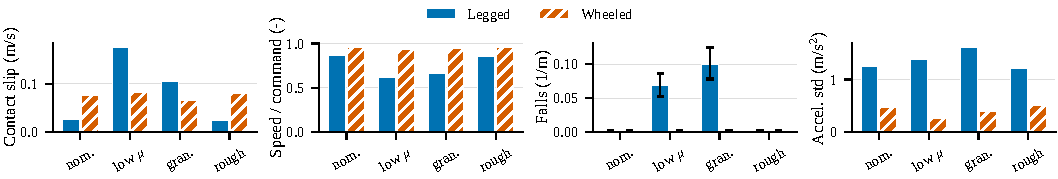
\includegraphics[width=\textwidth]{figures/fig2_configurations.pdf}
\caption{Dynamic behaviour by configuration and terrain, with 95\,\% credible intervals on falls. Wheeled slip and acceleration come from a different controller and contact geometry, and are not directly comparable with legged values.}
\label{fig:config}
\end{figure*}
\begin{figure*}[t]
\centering
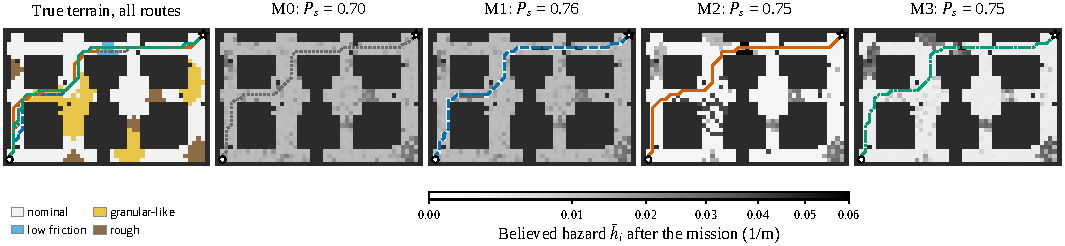
\includegraphics[width=\textwidth]{figures/fig4_risk_maps_trajectories.pdf}
\caption{One evaluation map (id 12, fixed in advance) at $\varepsilon=0.1$: true terrain with the four routes, and the hazard each method believes at mission end. Dots: start; stars: goal; dark cells: rock or high believed hazard. Here M1 happens to beat M2 and M3: the mean gain does not hold on every map.}
\label{fig:maps}
\end{figure*}

\emph{Monte Carlo.} Maps have $48\times32$ cells of 0.5\,m with drifts, crossings, rooms and pillars, and about \vhazFrac{}\,\% hazard coverage. Appearance is synthetic: per-map random prototypes with noise, so no terrain-to-look relation carries between maps; 15\,\% of hazard patches look like floor, and decoys make safe ground look hazardous. The Monte Carlo has no rendering, SLAM error or dynamics, and obstacles are known. Realised success draws one exponential threshold per replicate, shared across methods. Evaluation uses 200 maps with five replicates and common random numbers; the repetition uses 200 unseen maps. Parameters were tuned only on 50 development maps ($\sigma_k$=\vtunedKernelTwo{} for M2 and \vtunedKernelThree{} for M3, $\tau$=\vtunedTau{}, $\rho$=\vtunedRho{}, $\kappa$=\vtunedKappa{}; the last three at the edge of their grids). Fixed assumptions are $\lambda=25$, $\ell_w=1$\,m and hazard $[0.001,0.06,0.04,0.03]$\,m$^{-1}$ over $\mathcal{T}$, swept in Section~\ref{sec:sens}. In all, \vnMissionsTotal{} evaluation missions were run.

\emph{Statistics.} The map is the unit; replicates are averaged within it. We report 95\,\% bootstrap intervals of paired differences (10\,000 map resamples), Wilcoxon tests with Holm correction, and $d_z$. \sentbreak Hypotheses and refutation criteria were recorded before the campaigns: \textbf{H1} M2 beats M1 and M0; \textbf{H2} M1 beats M0; \textbf{H3} M3 beats M2; \textbf{H4} IMU plus joints beats each alone; \textbf{H5} the propagation gain differs between configurations through measured perception alone.

\section{Results and Discussion}
\subsection{Physical Behaviour}
The legged robot fell in \vfallsLegLow{} low-friction and \vfallsLegGran{} granular-like episodes and never on nominal or rough terrain, giving Jeffreys-posterior hazards of \vhLegLow{} and \vhLegGran{}\,m$^{-1}$, while contact slip rose from \vslipLegNom{} to \vslipLegLow{}\,m/s on low friction. The wheeled model never fell in 650 episodes, including ramps. The wheeled controller is ours, with a stiff stance, and has no fidelity claim, so the result describes these controllers only (Figs.~\ref{fig:mujoco} and~\ref{fig:config}).


\begin{figure*}[t]
\centering
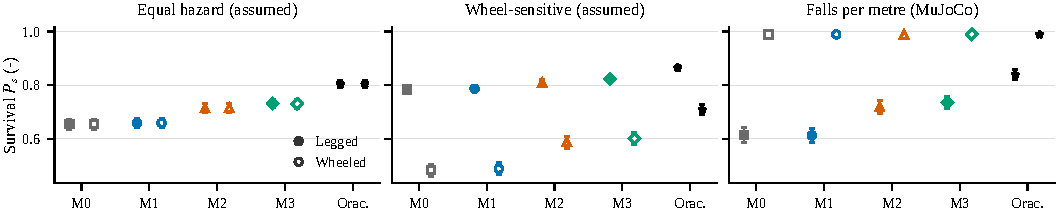
\includegraphics[width=\textwidth]{figures/fig3_measured_scenarios.pdf}
\caption{$P_s$ with measured classifier confusion (Fig.~\ref{fig:conf}) under three failure models (mean and 95\,\% interval, 200 maps). Filled: legged; open: wheeled. The configuration that gains most depends on the failure model.}
\label{fig:scen}
\end{figure*}
\begin{figure*}[t]
\centering
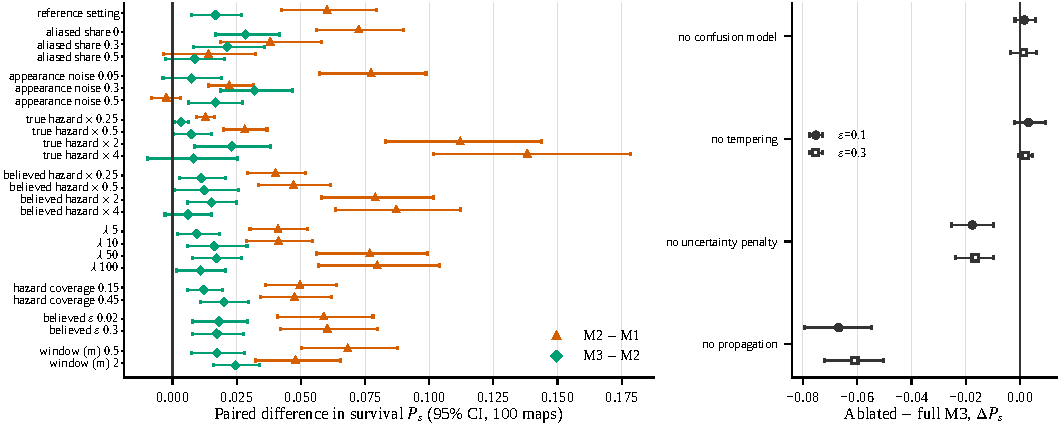
\includegraphics[width=\textwidth]{figures/fig8_sensitivity_ablation.pdf}
\caption{Left: sensitivity of the paired gains to assumed parameters at $\varepsilon=0.1$ (extremes of each sweep; the rest are in the repository). Right: ablation of M3 on 200 maps. Intervals crossing zero show no measurable effect.}
\label{fig:sens}
\end{figure*}

\subsection{Terrain Classification}
On \vnEpLeg{} legged and \vnEpWhe{} wheeled episodes (Table~\ref{tab:clf}), a random window split inflates legged macro-F1 from \vfOneLeg{} to \vfLeakLeg{}, which measures the leakage avoided. Held-out recall per class is \vrecLegNom{}, \vrecLegLow{}, \vrecLegGran{} and \vrecLegRough{} for nominal, low friction, granular-like and rough on the legged robot. Logistic regression does slightly better on the legged robot (\vfLogLeg{}, with lower calibration error); the forest stayed, as fixed in advance. H4 holds for the legged robot: fusion beats IMU by [\vfusImuLoLeg{}, \vfusImuHiLeg{}] and joints by [\vfusJointLoLeg{}, \vfusJointHiLeg{}]. For the wheeled robot the interval against IMU reaches zero, so H4 is not established there. The high scores say little about real ground: classes are separated by construction, and a wheeled F1 of \vfOneWhe{} mostly shows how clean simulated signals are. The stress tests are more informative. \sentbreak Mixed courses give \vfCourseLeg{} and \vfCourseWhe{}; with the legged robot, unseen speeds give as little as \vspeedLegMin{} (\vspeedLegLogMin{} with logistic regression) and unseen terrain parameters \vparamLegMin{}. Ramps, never trained on, are read as a hazard class in \vslopeHazardLeg{}\,\% (legged) and \vslopeHazardWhe{}\,\% (wheeled) of windows. The classifier interpolates within its training range and should not be trusted beyond it. Inference takes about \vinferMsLeg{}\,ms on a laptop core, not measured on the Jetson.

\begin{table}[!htb]
\centering
\caption{Classifier by Episode: Macro-F1 [95\,\% Interval] (Brier)}
\label{tab:clf}
\scriptsize
\resizebox{\columnwidth}{!}{\begin{tabular}{@{}lcc@{}}
\toprule
Macro-F1 (Brier score) & Legged & Wheeled \\ \midrule
IMU, forest & 0.939 [0.926, 0.951] (0.134) & 0.997 [0.995, 0.998] (0.015) \\
Joints, forest & 0.911 [0.895, 0.926] (0.178) & 0.990 [0.987, 0.993] (0.022) \\
IMU + joints, forest & 0.956 [0.943, 0.966] (0.102) & 0.998 [0.997, 0.999] (0.010) \\
IMU + joints, logistic & 0.963 [0.955, 0.970] (0.074) & 0.998 [0.997, 0.999] (0.004) \\
\midrule \multicolumn{3}{@{}l}{\emph{Stress tests, IMU + joints, forest}} \\
Random window split (leaky) & 0.982 & 0.999 \\
Held-out 20\,\% of episodes & 0.935 & 0.999 \\
Sensor noise $\times 3$ & 0.951 & 0.997 \\
Mixed terrain course & 0.820 & 0.842 \\
Unseen speed range (worse of two) & 0.450 & 0.963 \\
Unseen terrain parameters (worse of two) & 0.696 & 0.935 \\
\bottomrule
\end{tabular}}
\end{table}
\begin{figure}[!htb]
\centering
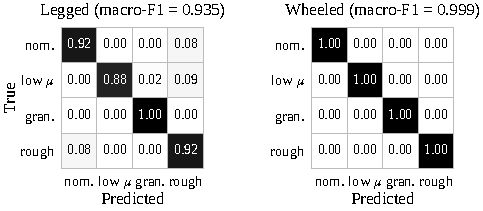
\includegraphics[width=\columnwidth]{figures/fig7_confusion.pdf}
\caption{Confusion on held-out episodes (fusion, forest), normalised by true class; source of the measured observation model.}
\label{fig:conf}
\end{figure}

\subsection{Map-Update Rules}
Tables~\ref{tab:main} and~\ref{tab:contrast} and Figs.~\ref{fig:maps} and~\ref{fig:robust} give the results. \textbf{H1 is supported}: at $\varepsilon=0.1$, M2 improves $P_s$ over M1 by \vdTwoOne{} [\vdTwoOneLo{}, \vdTwoOneHi{}], $d_z$=\vdTwoOneDz{}, and the repetition gives \vrepTwoOne{} [\vrepTwoOneLo{}, \vrepTwoOneHi{}]. Against M0, M2 and M3 cut the accumulated hazard by \vriskRedTwo{}\,\% and \vriskRedThree{}\,\%. The cost is \vlenAddTwo{}\,m of path and more replanning (\vrepMt{} against \vrepMo{} replans); a search took \vplanMsMt{}--\vplanMsMh{}\,ms on average in Python on a laptop. \textbf{H2 is not established}: M1 improves on M0 by only \vdOneZero{} [\vdOneZeroLo{}, \vdOneZeroHi{}], Holm-adjusted $p$=\vdOneZeroHolm{}, and the repetition interval [\vrepOneZeroLo{}, \vrepOneZeroHi{}] includes zero. Local updates arrive after the ground is crossed. \sentbreak A stronger baseline, added after internal review, also spreads evidence to cells within a 2\,m reach, by distance alone: it gains only \vspatialVsLocal{} [\vspatialVsLocalLo{}, \vspatialVsLocalHi{}] over M1, and M2 still beats it by \vspatialGain{} [\vspatialGainLo{}, \vspatialGainHi{}], so appearance, not mere spatial spread, carries the gain. \textbf{H3 is supported with a small effect}: M3 adds \vdThreeTwo{} [\vdThreeTwoLo{}, \vdThreeTwoHi{}] over M2, \vrepThreeTwo{} on repetition, growing with classifier error (\vdThreeTwoFive{} at $\varepsilon=0.5$). All methods stay well below the oracle bound of \vpsOrc{}.

\begin{table}[!htb]
\centering
\caption{Monte Carlo at $\varepsilon=0.1$, Equal Assumed Hazard (200 Maps, 95\,\% Bootstrap Intervals)}
\label{tab:main}
\scriptsize
\resizebox{\columnwidth}{!}{\begin{tabular}{@{}lcccrr@{}}
\toprule
Method & $P_s$ & Success & Exposure (m) & Path (m) & Replans \\ \midrule
M0 geometry & 0.654 [0.635, 0.671] & 0.676 & 9.10 [8.59, 9.61] & 32.6 & 0.0 \\
M1 local & 0.657 [0.639, 0.675] & 0.678 & 9.03 [8.52, 9.54] & 32.6 & 4.5 \\
M2 appearance & 0.712 [0.696, 0.729] & 0.728 & 7.35 [6.87, 7.83] & 33.0 & 19.5 \\
M3 fusion & 0.727 [0.712, 0.743] & 0.750 & 6.92 [6.47, 7.39] & 33.0 & 12.1 \\
Oracle (bound) & 0.804 [0.791, 0.817] & 0.824 & 4.73 [4.35, 5.14] & 33.4 & 0.0 \\
\bottomrule
\end{tabular}}
\end{table}
\begin{figure}[!htb]
\centering
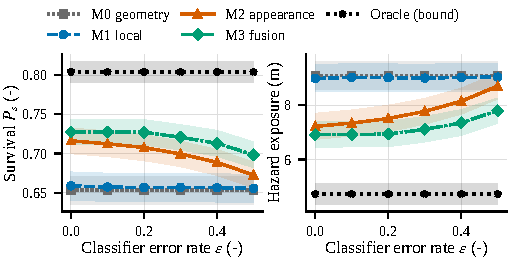
\includegraphics[width=\columnwidth]{figures/fig6_robustness.pdf}
\caption{Robustness to classifier error (mean and 95\,\% interval, 200 maps; synthetic symmetric confusion).}
\label{fig:robust}
\end{figure}
\begin{table}[!htb]
\centering
\caption{Paired Differences in $P_s$ [95\,\% Bootstrap Interval]}
\label{tab:contrast}
\scriptsize
\resizebox{\columnwidth}{!}{\begin{tabular}{@{}lccc@{}}
\toprule
Condition & M1 $-$ M0 & M2 $-$ M1 & M3 $-$ M2 \\ \midrule
Synthetic $\varepsilon$=0.1 & +0.004 [+0.000, +0.007] & +0.055 [+0.043, +0.067] & +0.015 [+0.008, +0.023] \\
Synthetic $\varepsilon$=0.3 & +0.003 [+0.001, +0.006] & +0.043 [+0.031, +0.054] & +0.021 [+0.015, +0.028] \\
Repeat, $\varepsilon$=0.1 & +0.001 [\mbox{$-$}0.002, +0.004] & +0.049 [+0.038, +0.059] & +0.014 [+0.008, +0.019] \\
Held-out conf., legged & +0.005 [+0.002, +0.008] & +0.055 [+0.043, +0.067] & +0.018 [+0.010, +0.027] \\
Held-out conf., wheeled & +0.005 [+0.002, +0.009] & +0.057 [+0.045, +0.070] & +0.015 [+0.005, +0.024] \\
Course conf., legged & +0.005 [+0.002, +0.008] & +0.044 [+0.033, +0.055] & +0.027 [+0.019, +0.036] \\
MuJoCo falls, legged & \mbox{$-$}0.002 [\mbox{$-$}0.007, +0.002] & +0.106 [+0.086, +0.127] & +0.016 [+0.003, +0.030] \\
MuJoCo falls, wheeled & +0.000 [\mbox{$-$}0.000, +0.000] & +0.000 [+0.000, +0.000] & +0.000 [\mbox{$-$}0.000, +0.000] \\
\bottomrule
\end{tabular}}
\end{table}

\subsection{Does the Benefit Depend on the Feet?}
With equal assumed hazards and only the measured confusion differing, the M2$-$M1 gain is \vintLegEqual{} (legged) and \vintWheEqual{} (wheeled). \sentbreak Their difference, \vintDiffEqual{} [\vintLoEqual{}, \vintHiEqual{}], excludes zero, so H5 survives its recorded criterion, but the effect is negligible: perception quality creates no meaningful difference between configurations. Fig.~\ref{fig:scen} shows what does. With an assumed table that penalises wheels, the gain is larger for wheels (\vintWheSens{} against \vintLegSens{}). With simulated falls per metre (Fig.~\ref{fig:config}), the ordering reverses: legged \vintLegFalls{}, wheeled \vintWheFalls{}, because wheeled $P_s$ is already \vfallPsWheMz{} under M0, a level set by the Jeffreys prior since no fall occurred. An unmeasured table should therefore not be used to claim that one configuration benefits more. Mixed-course confusion lowers the M2 gain while M3 holds (Table~\ref{tab:contrast}).

\subsection{Sensitivity and Ablation}\label{sec:sens}
The propagation gain depends on the assumed appearance channel (Fig.~\ref{fig:sens}): it falls from \valiasZero{} with no aliasing to \valiasHigh{} [\valiasHighLo{}, \valiasHighHi{}] when half the patches are aliased, and to \vnoiseHigh{} [\vnoiseHighLo{}, \vnoiseHighHi{}] at high appearance noise. It scales with hazard, from \vhzLow{} to \vhzHigh{} across a 16-fold range. In M3, removing the confusion model (\vabConf{} [\vabConfLo{}, \vabConfHi{}]) or the tempering (\vabTemper{} [\vabTemperLo{}, \vabTemperHi{}]) has no measurable cost, so these are not supported as contributors. Removing propagation costs \vabProp{} and the uncertainty penalty \vabUnc{}. A higher $\lambda$ partly replaces that penalty, but even with each method at its best swept $\lambda$, M3 exceeds M2 by \vbestBest{} [\vbestBestLo{}, \vbestBestHi{}] at $\varepsilon=0.1$, so the soft fusion appears to account for the persistent part. This sweep is descriptive.

\subsection{Implications and Limitations}
Three points follow, conditional on this simulation. First, a local update alone arrives too late to change the route; its value is as a source of labels. Second, propagation is only as good as the appearance channel, so the first measurement to make is how well the robot's cameras separate physically different terrains. Third, failure must be measured for each configuration with its real controller before claiming that one benefits more.

No result comes from the physical robot, and none validates a real mine. The Monte Carlo is algorithmic: appearance is synthetic, so H1 rests on an assumption that vision must earn, and work on real images~\cite{wellhausen2019,mattamala2025} is the better guide to it. Falls are a narrow notion of failure. Joint signals have not been captured from the robot, and the sim-to-real gap of the classifier is unknown and likely large. Gazebo produced no result here, since it follows the pose computed by MuJoCo; under ROS~2 Jazzy its wheeled motion gate failed (0.184\,m/s after release).

\FloatBarrier
\section{Conclusion}
In this simulation study, spreading proprioceptive evidence by appearance raised mission survival, while updating only the crossed ground did almost nothing. A soft, uncertainty-penalised fusion added a small gain that grew with classifier error. The failure model, not perception, decided whether the benefit favours legs or wheels. Next steps are capturing joint signals on the robot under supervision, replacing synthetic appearance with camera features, and measuring failure on real surfaces.

\section*{Reproducibility}
Code, per-mission records with their seeds, evaluation maps, window features and the scripts that regenerate every number, table and figure are available at \url{https://github.com/JoseSegundoM/proprioceptive_risk_mapping}. The robot models come from the project repository \texttt{mine\_sentinel\_autonomy}, and raw MuJoCo signals are regenerated from their recorded seeds.

\interlinepenalty=10000  % a reference is never split across columns
\bibliographystyle{IEEEtran}
\bibliography{references}

\end{document}
.
% Requires \PaperTitle, \PaperAuthors (UTF-8, hyperref) and \PaperAuthorsPDF
% (PDFDocEncoding octal escapes, \pdfinfo) to be defined first.
\ifdefined\PDFPROFILE\else\def\PDFPROFILE{ieee}\fi
\def\profileinteractive{interactive}
\usepackage{tikz}
\usetikzlibrary{svg.path}
\definecolor{orcidlogocol}{HTML}{A6CE39}
% ORCID iD logo, same artwork as the orcidlink package (vector, no Type 3).
\newlength{\orcidxheight}
\newcommand{\orcidlogo}{\setlength{\orcidxheight}{\fontcharht\font`X}%
  \mbox{\begin{tikzpicture}[yscale=-0.00390625*\orcidxheight,
      xscale=0.00390625*\orcidxheight,transform shape]
    \fill[orcidlogocol] svg{M256,128c0,70.7-57.3,128-128,128C57.3,256,0,198.7,0,128C0,57.3,57.3,0,128,0C198.7,0,256,57.3,256,128z};
    \fill[white] svg{M86.3,186.2H70.9V79.1h15.4v48.4V186.2z}
      svg{M108.9,79.1h41.6c39.6,0,57,28.3,57,53.6c0,27.5-21.5,53.6-56.8,53.6h-41.8V79.1z M124.3,172.4h24.5c34.9,0,42.9-26.5,42.9-39.7c0-21.5-13.7-39.7-43.7-39.7h-23.7V172.4z}
      svg{M88.7,56.8c0,5.5-4.5,10.1-10.1,10.1c-5.6,0-10.1-4.6-10.1-10.1c0-5.6,4.5-10.1,10.1-10.1C84.2,46.7,88.7,51.3,88.7,56.8z};
  \end{tikzpicture}}}
\ifx\PDFPROFILE\profileinteractive
  \usepackage[colorlinks=true,linkcolor=black,citecolor=black,urlcolor=blue,
              bookmarks=false]{hyperref}
  \hypersetup{pdftitle={\PaperTitle},pdfauthor={\PaperAuthors}}
  \newcommand{\orcid}[1]{\href{https://orcid.org/#1}{\orcidlogo}}
  \newcommand{\authoremail}[1]{\href{mailto:#1}{#1}}
  \newcommand{\doititle}[2]{\href{https://doi.org/#1}{#2}}
  \newcommand{\urltitle}[2]{\href{#1}{#2}}
\else
  \pdfinfo{/Title (\PaperTitle) /Author (\PaperAuthorsPDF)}
  \newcommand{\orcid}[1]{\orcidlogo}
  \newcommand{\authoremail}[1]{#1}
  \newcommand{\doititle}[2]{#2}
  \newcommand{\urltitle}[2]{#2}
\fi
